%----------------------------------------------------------------------------------------
%	PACKAGES AND OTHER DOCUMENT CONFIGURATIONS
%----------------------------------------------------------------------------------------

\documentclass[twoside,twocolumn]{article}

\usepackage{blindtext} % Package to generate dummy text throughout this template 
\usepackage[sc]{mathpazo} % Use the Palatino font
\usepackage[T1]{fontenc} % Use 8-bit encoding that has 256 glyphs
\usepackage{microtype} % Slightly tweak font spacing for aesthetics
\usepackage{amsmath,array,graphicx}
\usepackage{natbib}
\usepackage[intoc]{nomencl}
\usepackage[per-mode=symbol,exponent-product=\cdot,separate-uncertainty=true]{siunitx}
\usepackage{titling} % Customizing the title section
\usepackage[english]{babel} % Language hyphenation and typographical rules
\usepackage[hmarginratio=1:1,top=32mm,columnsep=20pt]{geometry} % Document margins
\usepackage[hang, small,labelfont=bf,up,textfont=it,up]{caption} % Custom captions under/above floats in tables or figures
\usepackage{booktabs} % Horizontal rules in tables
\usepackage{lettrine} % The lettrine is the first enlarged letter at the beginning of the text
\usepackage[figuresright]{rotating}
\usepackage{enumitem} % Customized lists
\usepackage{abstract} % Allows abstract customization
\usepackage{dblfloatfix} % allows figures to float in double columns
\usepackage{titlesec} % Allows customization of titles
\usepackage{fancyhdr} % Headers and footers
\usepackage{stackengine}
\usepackage{url}
\usepackage{wrapfig}
\usepackage{xfrac}
\usepackage[figuresright]{rotating}
\usepackage{longtable}
\usepackage{pdflscape}
\usepackage{mhchem}
\usepackage{subcaption}
\usepackage{stackengine}
\usepackage{url}
\usepackage{wrapfig}
\usepackage{blindtext}
\usepackage{enumitem}
\usepackage{blindtext}
\usepackage[raggedright]{sidecap}
\usepackage{wrapfig}
\usepackage[intoc]{nomencl}
\usepackage{float}
%\usepackage[active,floats,tightpage]{preview}
\usepackage{emptypage}
\usepackage{lipsum,afterpage}
\usepackage[a4,frame,center,noinfo]{crop}
\usepackage[strict]{changepage}
\usepackage{minitoc}
\DeclareSIUnit{\M}{M}
\DeclareSIUnit{\k}{k}
\DeclareSIUnit{\yrs}{yrs}
\usepackage{listofitems}


\linespread{1.05} % Line spacing - Palatino needs more space between lines
\setlist[itemize]{noitemsep} % Make itemize lists more compact

\renewcommand{\abstractnamefont}{\normalfont\bfseries} % Set the "Abstract" text to bold
\renewcommand{\abstracttextfont}{\normalfont\small\itshape} % Set the abstract itself to small italic text
\renewcommand\thesection{\Roman{section}} % Roman numerals for the sections
\renewcommand\thesubsection{\roman{subsection}} % roman numerals for subsections
\titleformat{\section}[block]{\large\scshape\centering}{\thesection.}{1em}{} % Change the look of the section titles
\titleformat{\subsection}[block]{\large}{\thesubsection.}{1em}{} % Change the look of the section titles

\pagestyle{fancy} % All pages have headers and footers
\fancyhead{} % Blank out the default header
\fancyfoot{} % Blank out the default footer
\fancyhead[C]{ANN-based modeling for wind-assist hydro-mechanics $\bullet$ Feb 2020 $\bullet$ Vol. XXI, No. 1} % Custom header text
\fancyfoot[RO,LE]{\thepage} % Custom footer text


\usepackage{hyperref} % For hyperlinks in the PDF
\usepackage[noabbrev, capitalise, nameinlink]{cleveref}

%----------------------------------------------------------------------------------------
%	TITLE SECTION
%----------------------------------------------------------------------------------------

\setlength{\droptitle}{-4\baselineskip} % Move the title up

\pretitle{\begin{center}\Huge\bfseries} % Article title formatting
\posttitle{\end{center}} % Article title closing formatting
\title{Machine Learning Based Hydro-mechanic Modeling for Sailing Commercial Ships} % Article title
\author{%
\textsc{Nico van der Kolk}\thanks{Corresponding author} \\[1ex] % Your name
\normalsize Blue Wasp Marine \\ % Your institution
\normalsize \href{mailto:nvanderkolk@bluewaspmarine.com}{nvanderkolk@bluewaspmarine.com} % Your email address
\and % Uncomment if 2 authors are required, duplicate these 4 lines if more
\textsc{Brian S. Freeman} \\[1ex] % Second author's name
\normalsize Lakes Environmental \\ % Second author's institution
\normalsize \href{brian.freeman@weblakes.com}{brian.freeman@weblakes.com } % Second author's email address
}
\date{} % Leave empty to omit a date
%\renewcommand{\maketitlehookd}{%
\begin{abstract}
\noindent 
The maturity of Reynolds-averaged Navier Stokes computational fluid dynamics (RANS-CFD) packages offers the ready assessment of the hydro-mechanic performance of a wind-assisted commercial ship. However, these simulations require intensive computational resources and complex software to generate results. In the hull optimisation context, individual adjustments to parameters require discrete processing that may take hours or days to process. To expedite results under different hull designs, or in the context of bulk analysis of multiple vessels in a fleet,  machine learning models are trained on a database of RANS-CFD for a systematic hull series. The model successfully trained on the RANS-CFD results with over 94\% accuracy for 60 different hull variations. Using the trained model to evaluate new runs on individual hulls showed over 86\% accuracies, allowing for rapid, accurate reproduction of vessel response for generic wind-assist hulls which can be quickly evaluated under a wide variety of sailing conditions. 
\end{abstract}
%}

%----------------------------------------------------------------------------------------

\begin{document}
\bibliographystyle{plain}
% !TeX root = ../dissertation.tex

%macros
\newcommand{\DWA}{\ensuremath{\mathrm{DWA}}\xspace}
\newcommand{\firstseries}{\ensuremath{1^{\mathrm{st}} \thinspace \text{Series}}\xspace}
\newcommand{\secondseries}{\ensuremath{2^{\mathrm{nd}} \thinspace\text{Series}}\xspace}
\newcommand{\thirdseries}{\ensuremath{3^{\mathrm{rd}}\thinspace \text{Series}}\xspace}

\newcommand{\Co}{\ensuremath{Co}\xspace}
\nomenclature{\Co}{Courant Number $U \frac{\Delta t}{\Delta x}$}
\newcommand{\PWASP}{\ensuremath{P_{\mathrm{WASP}}}\xspace}
\nomenclature{\PWASP}{Available wind-assist power [kW]}
%hydrostatics
\newcommand{\Lnab}{\ensuremath{L/\nabla^{\sfrac{1}{3}}}\xspace}
\nomenclature{\Lnab}{Length to displacement ratio}
\newcommand{\LB}{\ensuremath{L/B}\xspace}
\nomenclature{\LB}{Length to beam ratio}
\newcommand{\BT}{\ensuremath{B/T}\xspace}
\nomenclature{\BT}{Beam to draft ratio}
\newcommand{\TL}{\ensuremath{T/L}\xspace}
\nomenclature{\TL}{Draft to lenth ratio}
\newcommand{\Cp}{\ensuremath{C_\mathrm{P}}\xspace}
\nomenclature{\Cp}{Prismatic coefficient $\frac{A_{\mathrm{Midship}}}{LBT}$}
\newcommand{\Cb}{\ensuremath{C_\mathrm{B}}\xspace}
\nomenclature{\Cb}{Block coefficient $\frac{\nabla}{LBT}$}
\newcommand{\Cm}{\ensuremath{C_\mathrm{M}}\xspace}
\nomenclature{\Cm}{Midship coefficient $\frac{A_{\mathrm{Midship}}}{BT}$}
\newcommand{\Cwp}{\ensuremath{C_\mathrm{WP}}\xspace}
\nomenclature{\Cwp}{Waterplane coefficient $\frac{A_\mathrm{WP}}{LB}$}
\newcommand{\Awpsw}{\ensuremath{A_\mathrm{WP}/S_\mathrm{Wet}}\xspace}
%\nomenclature{\Awpsw}{Waterplane area to wetted surface area ratio}
\newcommand{\Alat}{\ensuremath{A_\mathrm{Lat}}\xspace}
\nomenclature{\Alat}{Lateral area $Lt$}
\newcommand{\RbT}{\ensuremath{\frac{R_\mathrm{b}}{T}}\xspace}
\nomenclature{\RbT}{Bilge radius to draft ratio}
\newcommand{\hRb}{\ensuremath{\frac{h}{R_\mathrm{b}}}\xspace}
\nomenclature{\hRb}{Keel height to bilge radius ratio}

\newcommand{\TWA}{\ensuremath{TWA}\xspace}
\nomenclature{\TWA}{True wind angle (vessel reference frame) [degree]}
\newcommand{\TWD}{\ensuremath{TWD}\xspace}
\nomenclature{\TWD}{True wind direction (Earth reference frame) [degree]}
\newcommand{\TWS}{\ensuremath{TWS}\xspace}
\nomenclature{\TWS}{True wind speed [knots]}
\newcommand{\Fn}{\ensuremath{Fn}\xspace}
\nomenclature{\Fn}{Froude Number}
\newcommand{\Xs}{\ensuremath{X_\mathrm{Sail}}\xspace}
\nomenclature{\Xs}{Aerodynamic thrust generated by the WASP propulsor [kN]}

\newcommand{\Xtot}{\ensuremath{X_\mathrm{Tot}}\xspace}
\nomenclature{\Xtot}{Total resistance (including windage) [kN]}
\newcommand{\delrud}{\ensuremath{\delta_\mathrm{Rud}}\xspace}
\nomenclature{\delrud}{Rudder angle [degree]} 

\newcommand{\Fx}{\ensuremath{X}\xspace}
\nomenclature{\Fx}{Flow-aligned component of vessel body force [kN]}
\newcommand{\Fy}{\ensuremath{Y}\xspace}
\nomenclature{\Fy}{Flow-normal component of vessel body force[kN]}
\newcommand{\Mz}{\ensuremath{N}\xspace}
\nomenclature{\Mz}{Vessel yawing moment [kNm]}

%modeling

\newcommand{\Rt}{\ensuremath{R_{\mathrm{Tot}}}\xspace}
\nomenclature{\Rt}{Total hydro-mechanic resistance [kN]}
\newcommand{\Xind}{\ensuremath{X_{i}}\xspace}
\nomenclature{\Xind}{Resistance due to sideforce production [kN]}
\newcommand{\Xphi}{\ensuremath{X_{\phi}}\xspace}
\nomenclature{\Xphi}{Resistance due to vessel heel [kN]}
\newcommand{\Xphiphi}{\ensuremath{X_{\phi\phi}}\xspace}
\nomenclature{$q$}{Dynamic pressure used for non-dimensionalisation}

\newcommand{\Cx}{\ensuremath{C_{X}}\xspace}
\nomenclature{\Cx}{Non-dimensional coefficient for resistance}
\newcommand{\Cxo}{\ensuremath{C_{XO}}\xspace}
\nomenclature{\Cxo}{Non-dimensional coefficient for resistance at zero-degrees leeway ($C_T$)}
\newcommand{\Xbb}{\ensuremath{X_{\beta \beta}}\xspace}
\nomenclature{\Xbb}{Maneuvring coefficient for resistance at leeway (second-order)}
\newcommand{\TeT}{\ensuremath{\sfrac{T_\mathrm{e}}{T}}\xspace}
\nomenclature{\TeT}{Vessel Effective draft (non-dimensionalised with draft $T$)}
\newcommand{\Te}{\ensuremath{T_\mathrm{e}}\xspace}
\newcommand{\ARe}{\ensuremath{AR_\mathrm{eff}}\xspace}
\nomenclature{\ARe}{Effective aspect ratio}
\newcommand{\ke}{\ensuremath{KE^\mathrm{'}}\xspace}

\newcommand{\nY}{\ensuremath{n_\mathrm{Y}}\xspace}
\newcommand{\Cy}{\ensuremath{C_\mathrm{Y}}\xspace}
\nomenclature{\Cy}{Non-dimensional coefficient for sideforce (Sway)}
\newcommand{\Yb}{\ensuremath{Y_{\beta}}\xspace}
\newcommand{\Yphi}{\ensuremath{Y_{\phi}}\xspace}
\nomenclature{\Yb}{Linear maneuvring coefficient for sideforce at leeway}
\newcommand{\Ybbb}{\ensuremath{Y_{\beta \beta \beta}}\xspace}
\nomenclature{\Ybbb}{Non-linear maneuvring coefficient for sideforce at leeway (third-order)}
\newcommand{\Ylin}{\ensuremath{Y_\mathrm{lin}}\xspace}
\newcommand{\Ynonlin}{\ensuremath{Y_\mathrm{non-lin}}\xspace}
\newcommand{\Yn}{\ensuremath{Y_n}\xspace}
\nomenclature{\Yn}{Sectional sideforce [kN/m]}
\newcommand{\Cyn}{\ensuremath{C_{\Yn}}\xspace}
\nomenclature{\Cyn}{Sectional sideforce coefficent $\frac{\Yn}{q\Tn d\xi}$}
\newcommand{\Tn}{\ensuremath{T_n}\xspace}
\nomenclature{\Tn}{Local draft [m]}


\newcommand{\Cn}{\ensuremath{C_\mathrm{N}}\xspace}
\newcommand{\Nb}{\ensuremath{N_{\beta}}\xspace}
\newcommand{\Nphi}{\ensuremath{N_{\phi}}\xspace}
\newcommand{\Nbbb}{\ensuremath{N_{\beta \beta \beta}}\xspace}
\newcommand{\Nlin}{\ensuremath{N_\mathrm{lin}}\xspace}
\newcommand{\Nnonlin}{\ensuremath{N_\mathrm{non-lin}}\xspace}
\nomenclature{\Cn}{Non-dimensional coefficient for yaw}
\nomenclature{\Nb}{Linear maneuvring coefficient for yaw at leeway}
\nomenclature{\Nbbb}{Non-linear maneuvring coefficient for yaw at leeway (third-order)}

\newcommand{\CLR}{\ensuremath{CLR}\xspace}
\newcommand{\dCLR}{\ensuremath{\sfrac{\partial\CLR}{\partial\beta}}\xspace}
\nomenclature{\CLR}{Center of lateral resistance [m]}
%-----------------------------------------------------------------------------------------


%-----------------------------------------------------------------------------------------


% Print the title
\maketitle

%----------------------------------------------------------------------------------------
%	ARTICLE CONTENTS
%----------------------------------------------------------------------------------------

\printnomenclature

\section{Introduction}

\lettrine[nindent=0em,lines=3]{W}ind assisted ship propulsion stands apart among available technologies for the energy transition in commercial shipping. A wind-hybrid vessel promises to deliver substantial fuel savings, a result that has been reported by several researchers in recent years \cite{Fujiwara05a, Naaijen10, Traut14, Eggers16}. This promise of substantial reductions in emissions, for both local pollutants and for greenhouse gases, is achievable in the near-term.

\begin{figure*}[!ht]
	\centering
	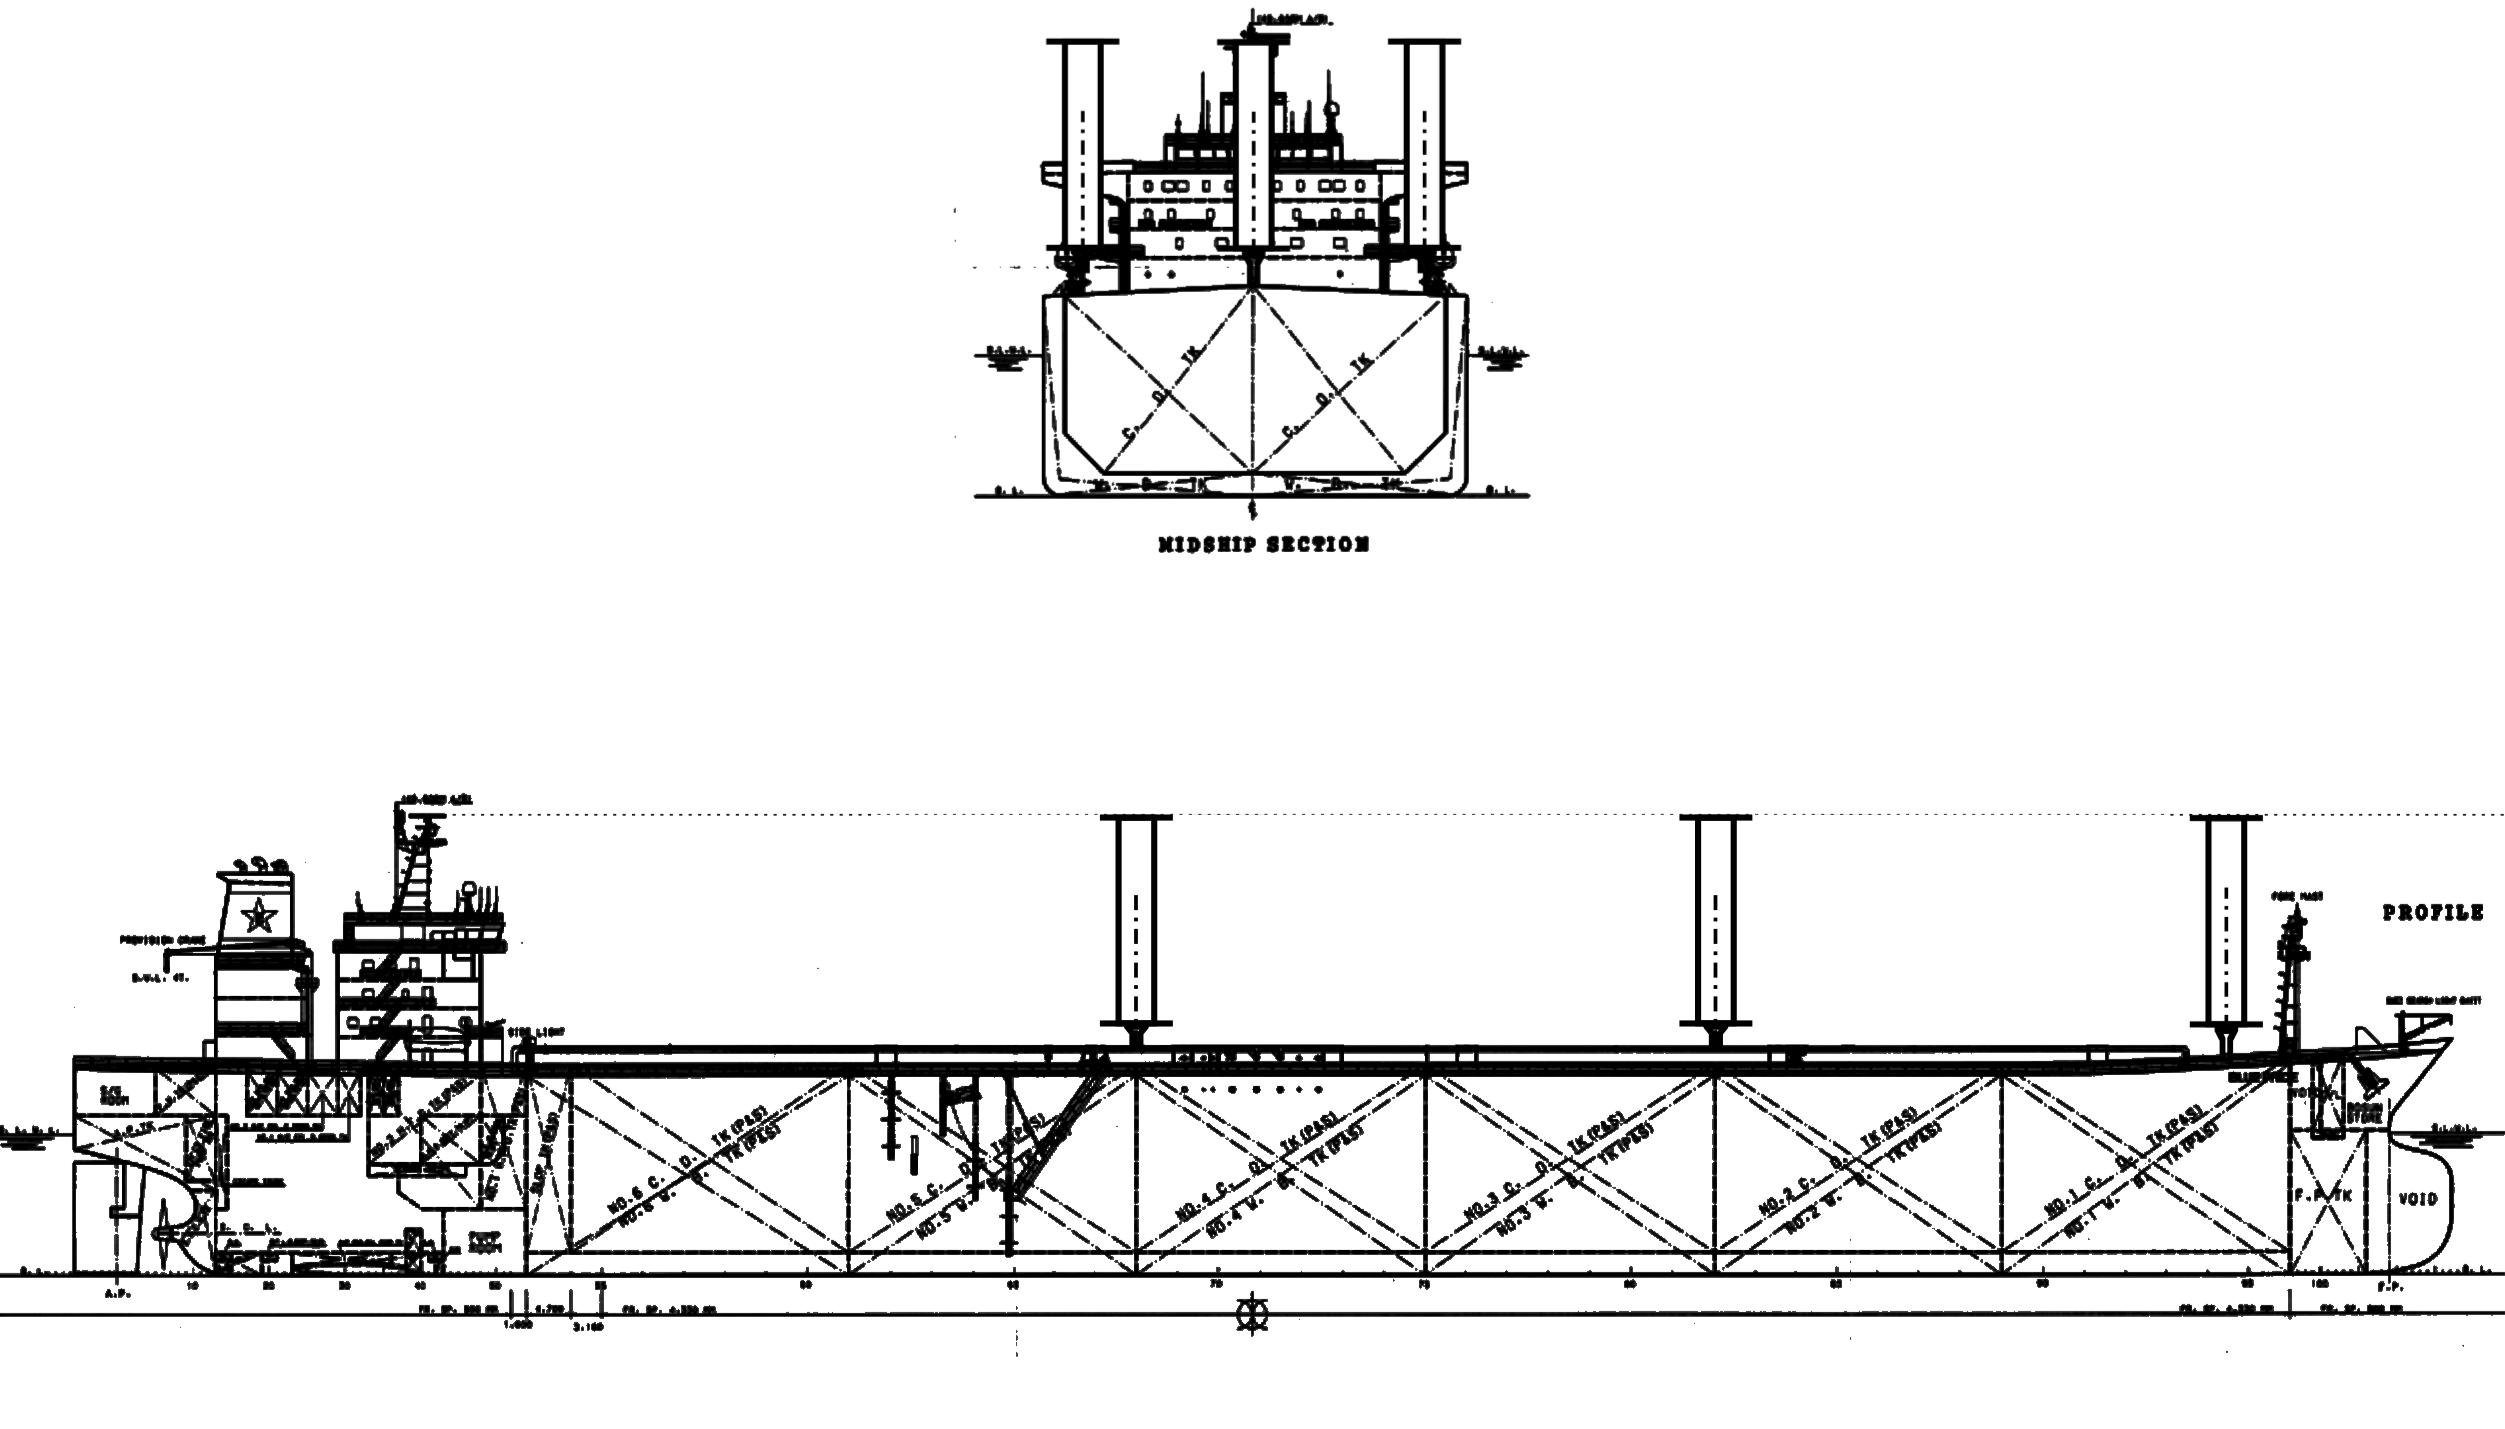
\includegraphics[width=\textwidth]{images/Panamax530.png}  %assumes jpg extension
	\caption{80,000 DWT Panamax bulker with three 30-meter Flettner rotors.}
	\label{fig:Panamax}
\end{figure*}

Technological readiness of wind assist concepts is not the barrier to broader market uptake. Several viable concepts for wind propulsors are commercially available. Rather, it is a lack of experience with industrialized sailing and unwillingness to take risk as an 'early adopter'. The further development of this promising technology is hampered by a poor understanding of  the interaction effects between wind propulsors and the hydro-mechanics of commercial ships. For the ship owner or operator, this lack of experience with industrial sailing introduces uncertainty in a profoundly risk-averse sector. For the regulator who wishes to promote the uptake of sustainable technologies, the knowledge gap raises the spectre of misdirected policies that fail to advance wind assisted ship propulsion as a viable component of the energy transition. In fact, wind propulsion is one of the only interventions in the maritime shipping sector that promises significant reductions in greenhouse gas emissions in the near term. Furthermore, besides the simple arithmetic of fuel savings and limiting exposure to increasingly volatile fuel prices, wind-assistance raises the possibility of engaging with an activist consumer class and potentially increasing the perceived value of shipped products.

\subsection{Wind-assist vessel model}
The reliable performance prediction of a wind-assisted ship is a necessary prerequisite for any sound economic and environmental evaluation of these concepts. Recognizing a general lack of understanding about the physics of wind-assist vessels, and the need for an assessment tool to facilitate the further development of this promising technology, a performance prediction tool is being developed by the Sail Assist research group. A quick yet reliable way to assess the performance of different wind-assisted ships will be useful throughout the design process. In early stages, when the user wants to explore several different designs, the in-built force models under development at Delft University of Technology may be used. In a more advanced design phase, the user can input data obtained by dedicated simulations or experiments. In this case the modeling tool is used purely as a solver to obtain very detailed results for a specific design.

%\begin{figure}[!th]
%	\centering
%	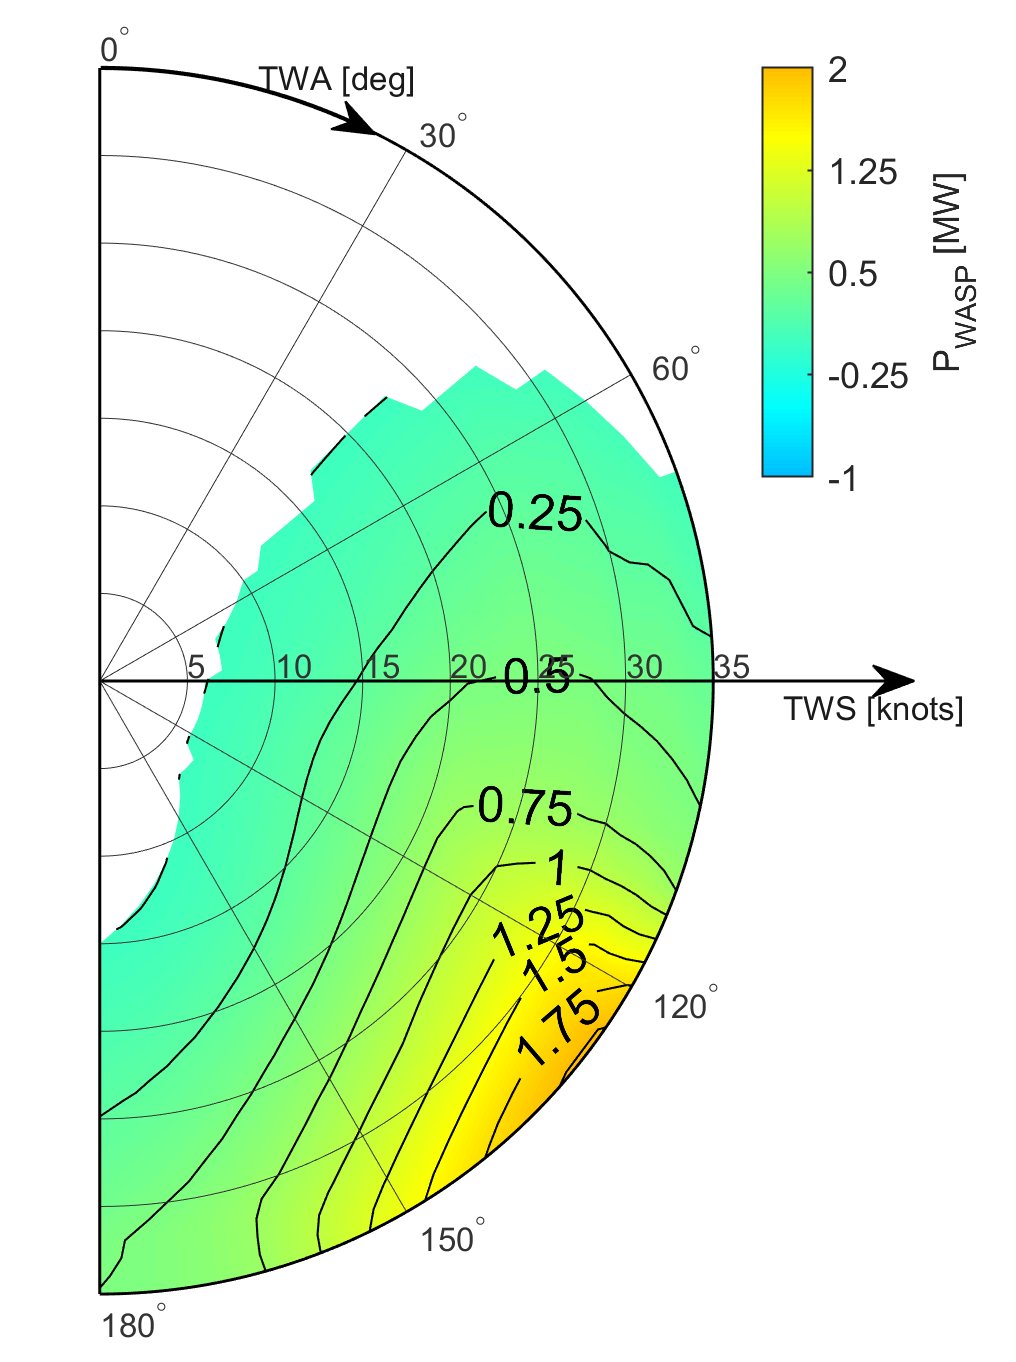
\includegraphics[width=\columnwidth]{images/P_Baltic224_10kts}
%	\caption{Available wind-assist power, \PWASP, for the Baltic test case CF5000-318 (10 knots).}
%	\label{fig:Pwasppolar}
%\end{figure}

The fundamental task of the performance prediction tool is to balance the aerodynamic and hydrodynamic forces acting on a wind-assisted ship to arrive at a sailing equilibrium. This is done within an optimization routine that minimizes the engine delivered thrust, $T(1-t)$, while maintaining a prescribed vessel speed. Alternative optimization routines may include pure sailing, delivering nominal engine power and maximizing speed, or maintaining a minimum speed. The program will calculate the performance of the wind-assisted ship for a specified range of true wind angle and true wind speed. 
%For example, the available wind-assist power, \PWASP, is plotted in \cref{fig:Pwasppolar} for the 5000 DWT DAMEN combi-freighter fitter with three 18-meter Flettner rotors (\cref{fig:Baltic318}). 

\PWASP considers the wind-assist propulsive power against any power needed to operate the wind propulsor. It is defined as:

\begin{equation}
\PWASP=\frac{V_{\mathrm{ref}}}{\eta_{\mathrm{T}}} \left( \Fx_{\mathrm{Aero}}-\Delta R_{\mathrm{Sailing}} \right) -\frac{P_{\mathrm{Rotor}}}{\eta_{\mathrm{Gen}}}
\label{eq:Pwasp}
\end{equation}

A design can be evaluated and improved based on these polar diagrams, or this information can be passed to a weather routing program or used to define the control systems of the wind propulsor. Finally, vessel performance with wind assist operation can be optimized, and studied for environmental impact and economic investment evaluations.

\section{Methodology}

\subsection{Modeling for hydro-mechanic response}

The ship adopts a heel and leeway angle to support the sail-plan. This combination places the hull---which is otherwise optimized for quite specific and symmetric operating conditions---oblique to the mean flow in the \textit{sailing condition}. The normal wave field produced as part of the wake of this ship will be superimposed on the pressure distribution arising from the sideforce production by the hull, along with the Munk yawing moment \cite{Munk1924}. Finally, a vessel heeling angle will bring the vessel "shoulders" closer to the free surface, leading to a further distortion of the wave system. The pressure resistance for a sailing ship will therefore vary with heel and leeway angles, alongside the ordinary Froude number dependency.

\begin{figure*}[!h]
	\centering
	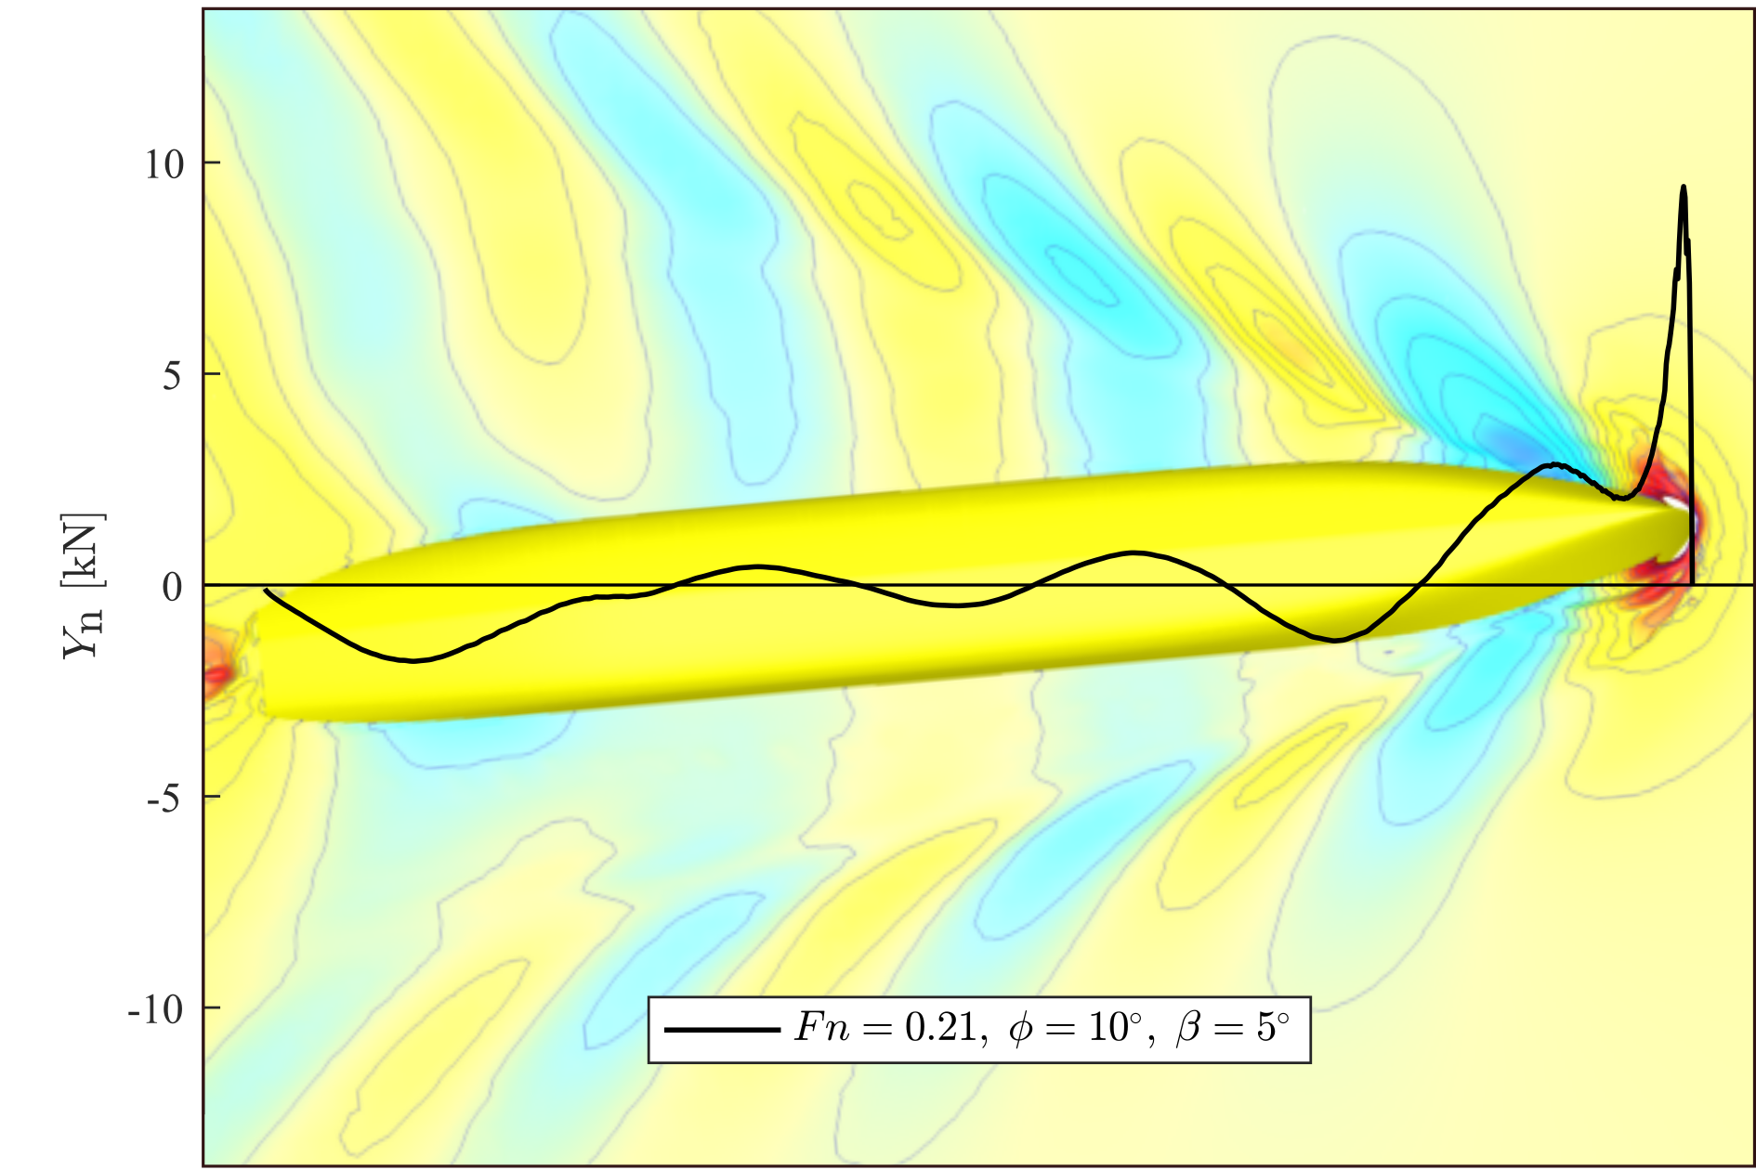
\includegraphics[width=.7\textwidth]{images/hull1.png}  %assumes jpg extension
	\caption{Distribution of hydrodynamic sideforce, showing wave system (viewpoint is below the ship).  Hull \# 1, leeway angle $\beta=\ang{5}$, heel angle $\phi=\ang{10}$. As the vessel heels, the fore and aft shoulders are brought close to the free surface, causing flow constriction and acceleration. This effect is especially pronounced at large heel angles ($\phi$=\ang{10} is normally adopted as operational limit for manned vessels).}
	\label{fig:Ynphi}
\end{figure*}

%\begin{figure*}[!th]
%	\centering
%	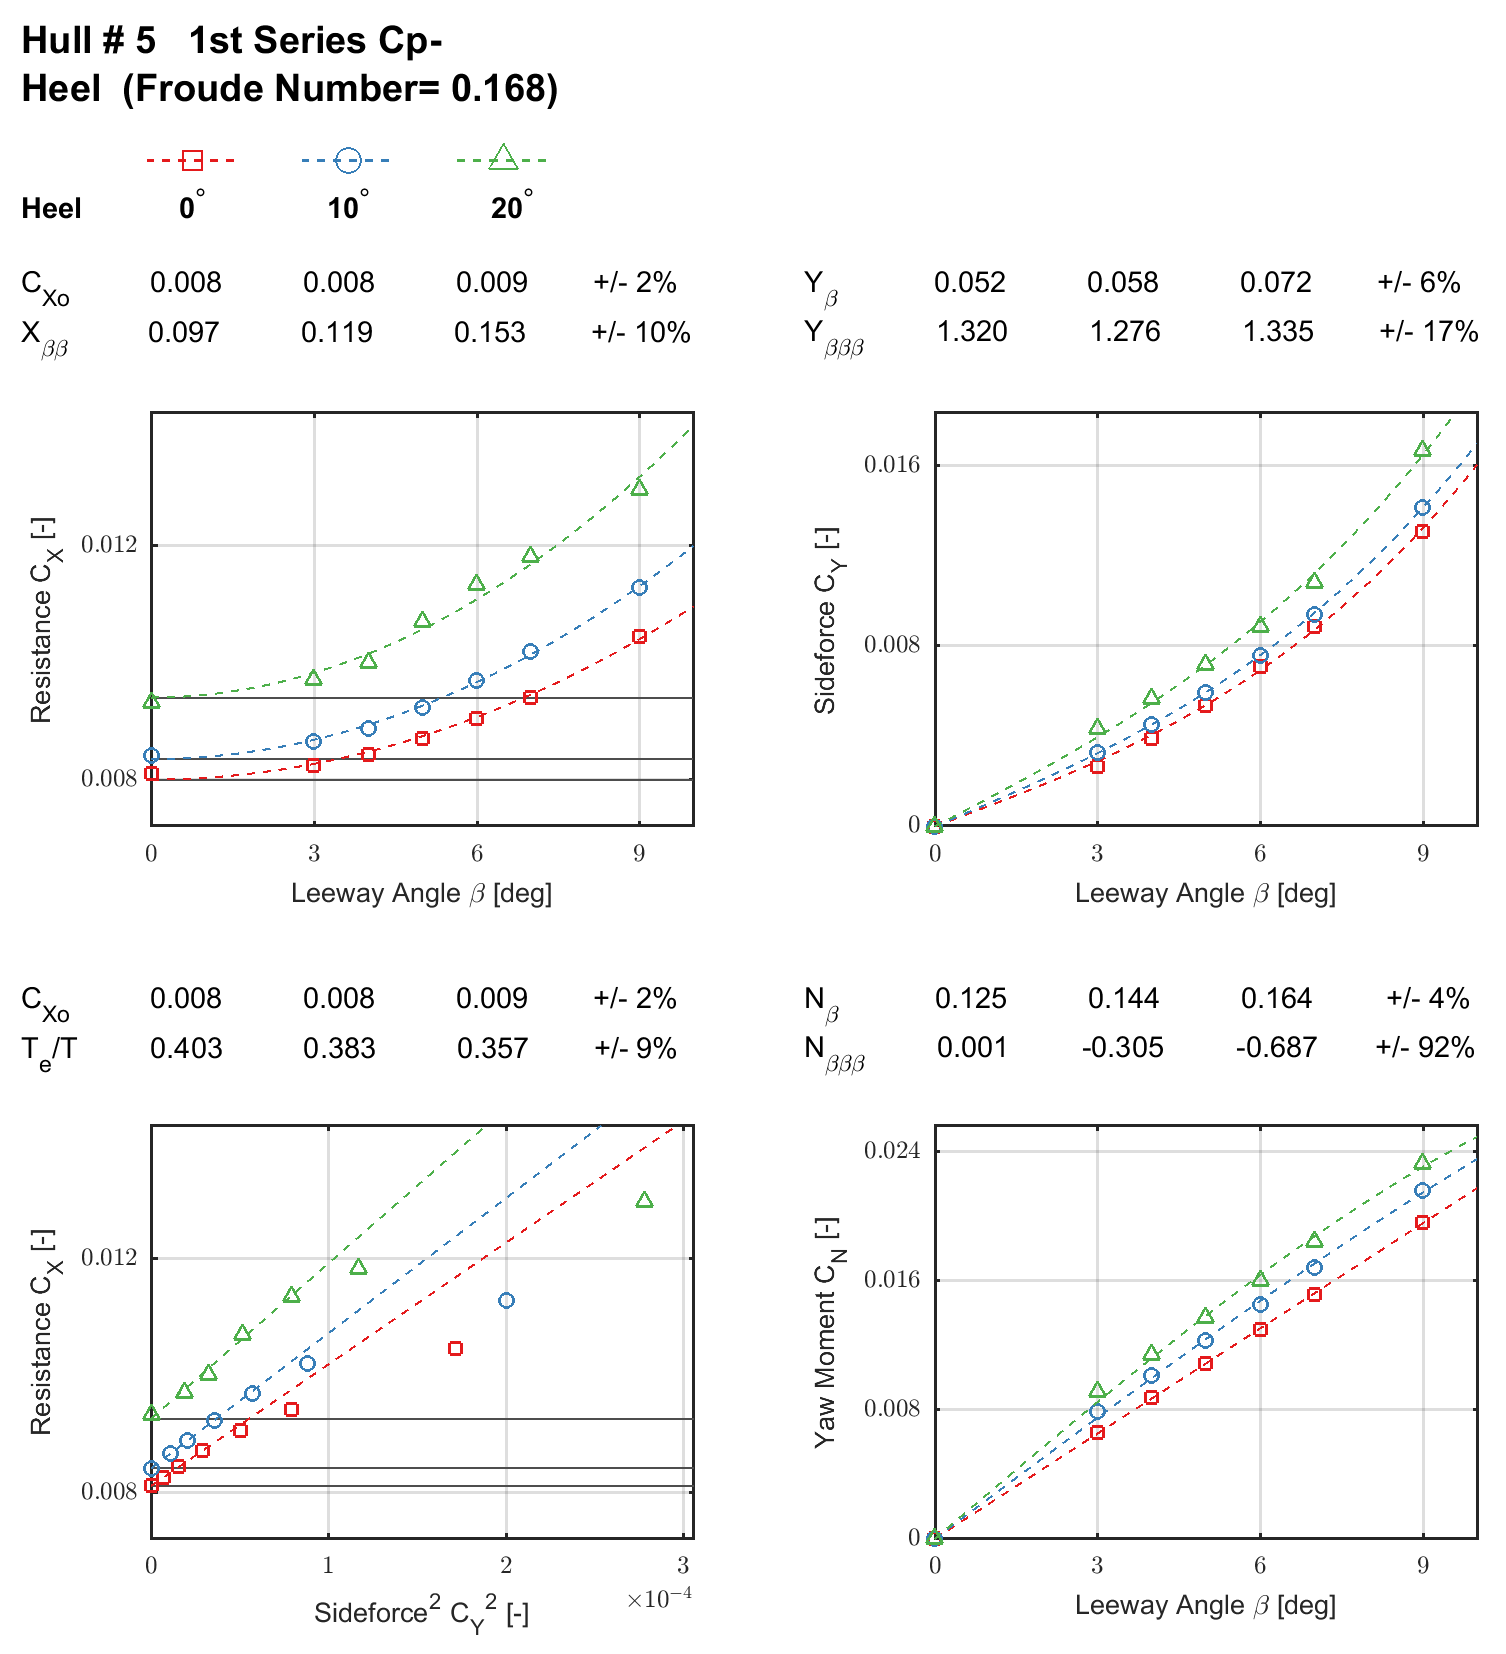
\includegraphics[width=\textwidth]{images/5heel_process}
%	\caption{Resistance increase for heel $\phi$ and leeway $\beta$ for hull \#5 of the \firstseries.}
%	\label{fig:5heel}
%\end{figure*}

The sailing performance for wind-assisted ships is synonymous with maneuvering forces for the steady drift condition, including vessel heel angle. A right hand rule is adopted with the $z$ axis pointed down. All rotations are performed about midship at the calm water line. Forces and moments are presented in flow-aligned coordinates, $<x,y>$, with the suitable transformation as in \cref{fig:cutcoord}.

\begin{figure}[!ht]
	\centering
	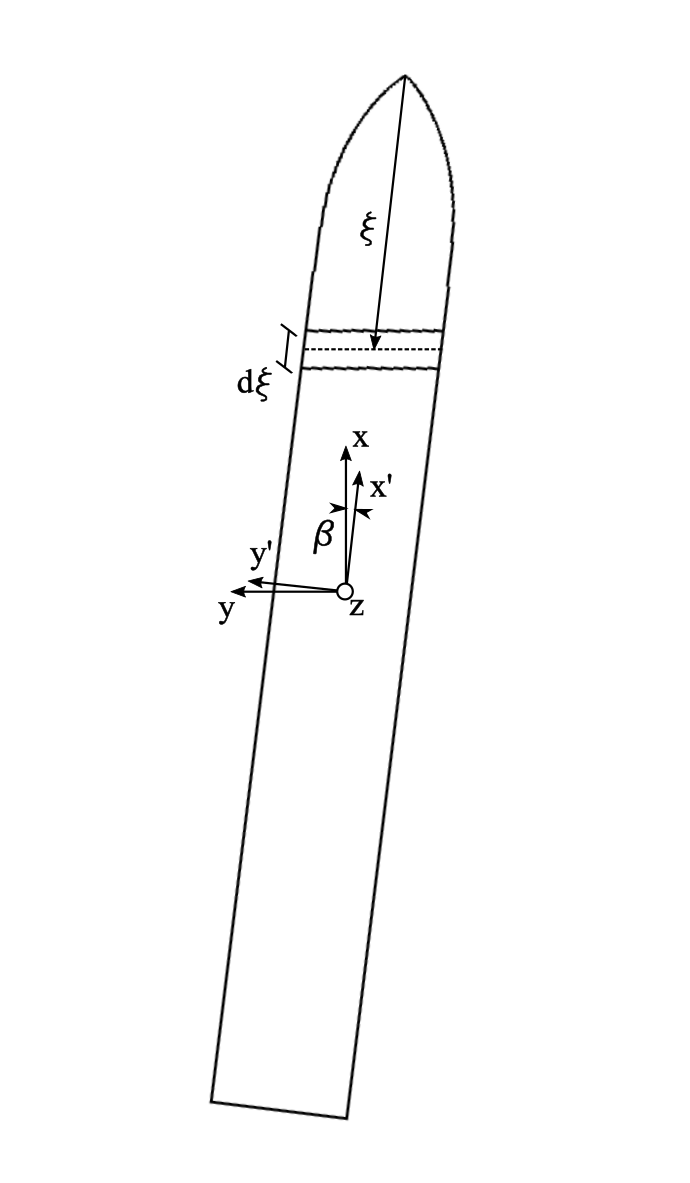
\includegraphics[width=.7\columnwidth]{images/cut_coordinates.png}  %assumes jpg extension
	\caption{Coordinate system for vessel hydro-mechanic response (viewpoint is below the ship).}
	\label{fig:cutcoord}
\end{figure}

The distribution of hydrodynamic sideforce (Sway) along the hull was extracted from simulation results. The field results for fluid pressure $\mathbf{P}$ and shear stress $\mathbf{S}$ are projected in the flow-normal direction (\nY) and integrated on segments of the hull (as in \cref{fig:cutcoord}).

\begin{equation}
\Yn=\int_{\xi}^{\xi+d\xi} \int_{z=0}^{\Tn} \left(\mathbf{P}+\mathbf{S}\right)  \cos{\beta} \space dz \space d\xi
\end{equation}

\subsubsection{Sailing efficiency}
For modeling of wind-assist vessels, the resistance increase due to the sailing condition (heel angle $\phi$, and leeway angle $\beta$) is expressed as an effective draft \Te. This quantity is related to the slope of a linear fit through data for several heel and leeway angles (bottom-left in \cref{fig:5heel}).

Following theories for low-aspect planforms \cite{Hoerner1985,Jones1946}, this induced drag may be significant for commercial ships, meaning that the thrust delivered by a wind propulsor might well be overwhelmed by this increase in resistance. Though the flow mechanisms only vaguely resemble the Prandtl lifting-line and the associated derivation for the induced drag \cite{Prandtl1918}, the accounting for energy loss in shed vorticity is especially relevant for the present application. Following the analysis of sailing yachts by \citet{Gerritsma1992}, the resistance increase due to sideforce production is modeled as an effective draft, $T_{e}$ \cite{Gerritsma1993}, which is a metric for the sailing efficiency of the hull. The expression is derived from the lifting-line theory of wings. In non-dimensional form:

\begin{subequations}
	\begin{align}
	\Cx&=\frac{1}{\pi \ARe}\Cy^2+\Cxo 
	\label{eq:CDi}\\
	\Te&=\sqrt{\dfrac{TL\xspace\ARe}{2}} 
	\label{eq:Te}
	\end{align}
\end{subequations}

\noindent
Forces and moments are non-dimensionalized using the dynamic pressure $q=\frac{1}{2}\rho U^2 $ following the maneuvering convention. A linear and thrid order term are assumed for $\beta$, and a linear term for $\phi$. The \ARe, as in \cref{eq:CDi} is derived from a (linear) curve fit. A non-dimensional form for the effective draft \Te is made with the vessel draft: \TeT \cref{eq:Te}, providing a convenient metric for the sailing efficiency of the hull. Some difficulty arises on account of the non-linear response of the commercial ship hull.

\subsubsection{Vessel course keeping ability}
The second quantity of principal interest for this modeling for wind-assist vessels is the center of effort for the distribution of lateral force, also known as the center of lateral resistance. The position of the \CLR is determined as the quotient of the yaw moment and the sideforce.

\begin{equation}
CLR=\sfrac{\Cn}{\Cy}
\end{equation}

\noindent
Again, body forces are non-dimensionalized with the dynamic pressure $q$.


\begin{equation}
\Cx=\Xbb\beta^{2}+\Xphi\phi
\end{equation}
\begin{equation}
\Cy=\Yb\beta+\Ybbb\beta^{3}+\Yphi\phi
\end{equation}
\begin{equation}
\Cn=\Nb\beta+\Nphi\phi
\end{equation}

Behavior for the \CLR as function of leeway angle $\beta$ is shown in \cref{fig:CLRdemo} for several appendage configurations: the bare hull (un-appended), the nominal appended hull design with rudder set for zero degrees, a short bilge keel in the most forward position, and a long bilge keel occupying the full length of the parallel midbody. The \CLR is given for leeway angles $\beta$ of three, six, and nine degrees. 

\begin{figure*}[!th]
	\centering
	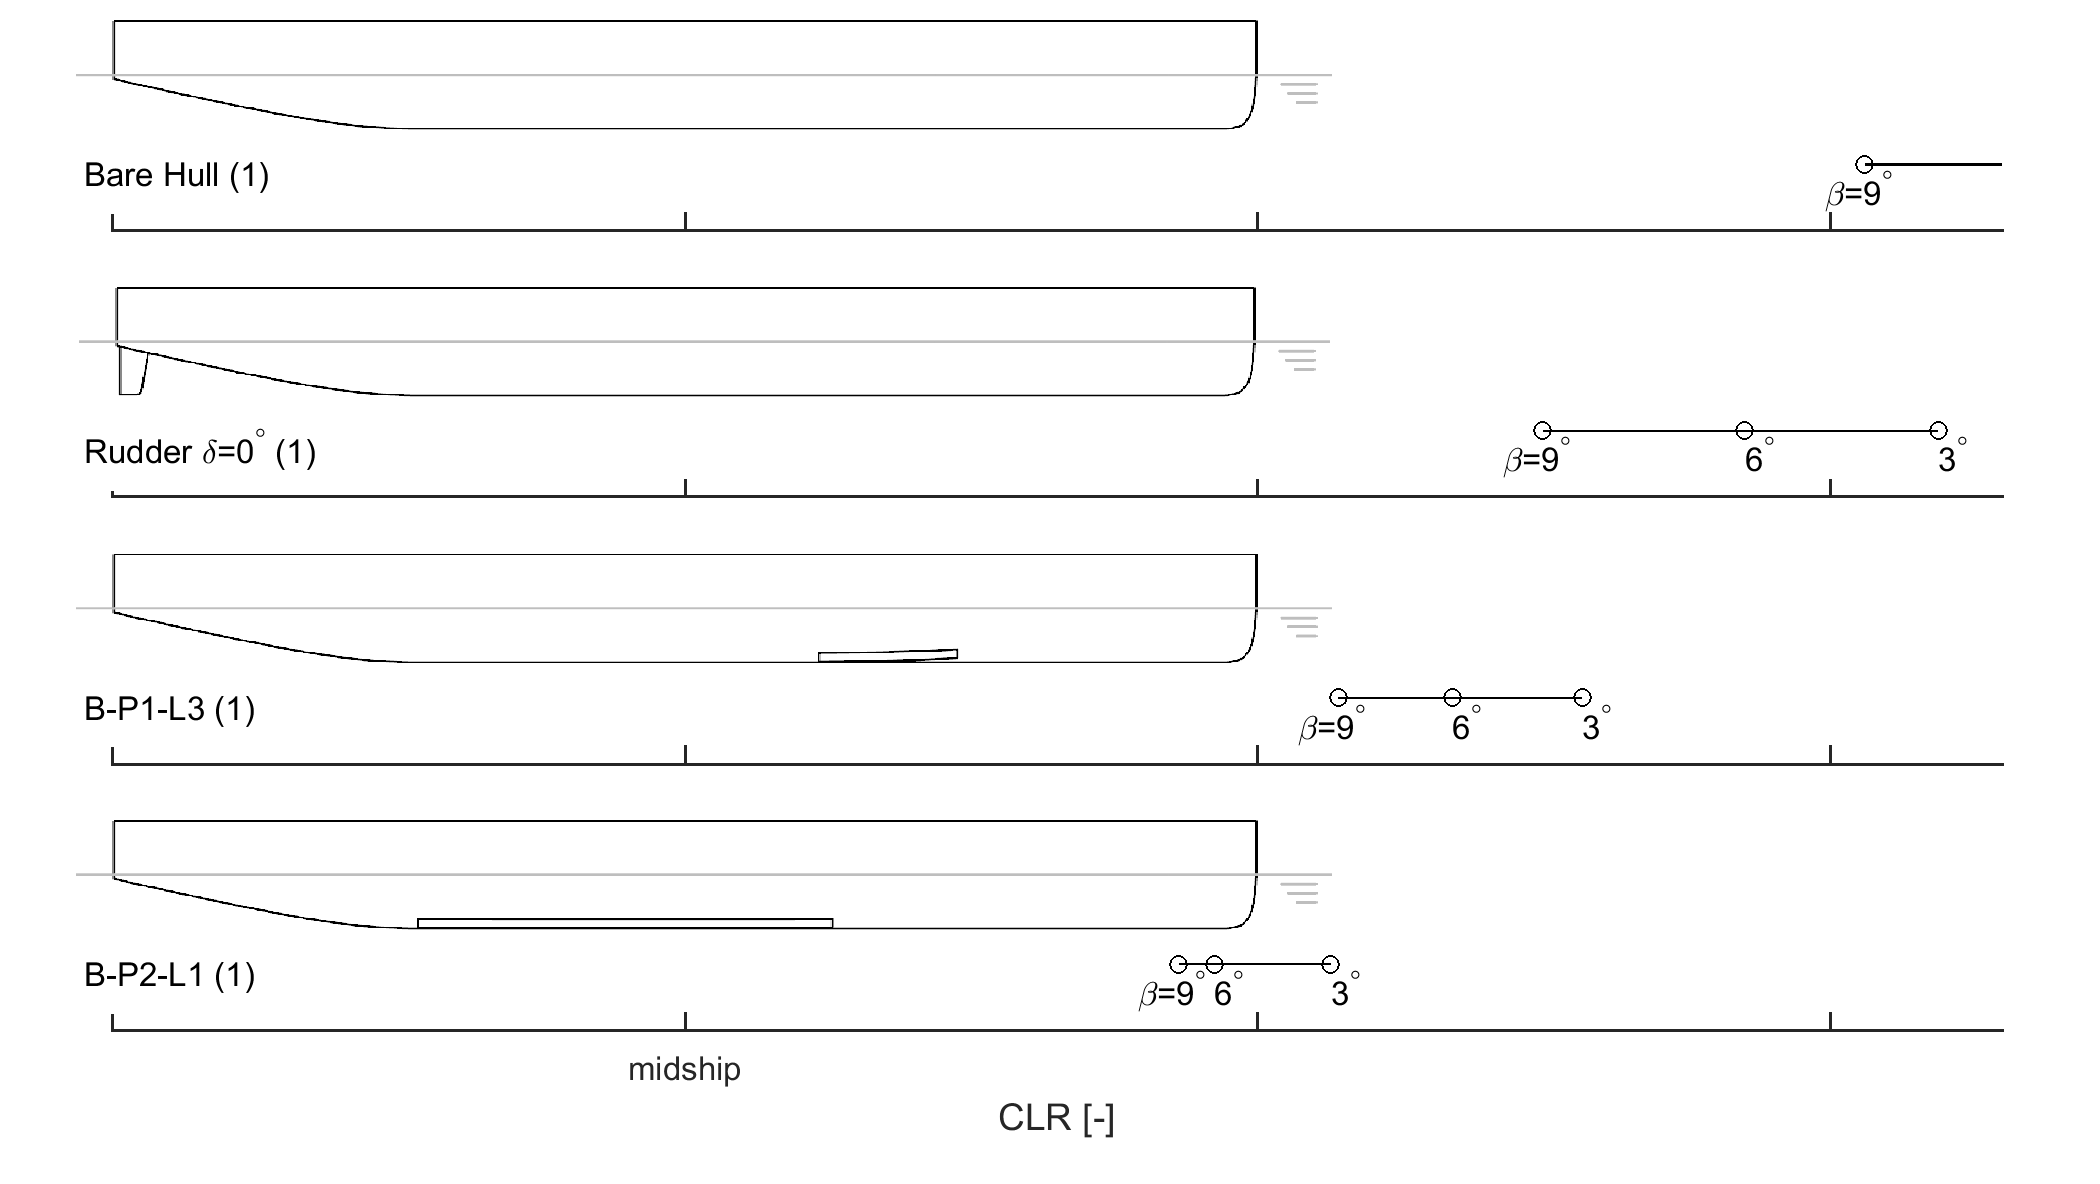
\includegraphics[width=\textwidth]{images/1_CLR_demo}
	\caption{Vessel \CLR for several appended hulls. Experimental result.}
	\label{fig:CLRdemo}
\end{figure*}
\noindent
First, observe the \CLR for the un-appended hull, which lies more than half a ships-length ahead of the bow (shown only for nine degrees leeway), a consequence of the stronger development of the yawing moment—linear with leeway angle—compared against the sideforce, which includes a significant higher-order dependency for leeway angle. The \CLR moves aft as the leeway angle increases, an effect that is driven by an increase in flow separation along the bilges. This effect is manifest as a rising contribution for the higher-order sideforce term in the sway equation, and an attenuation of the “Munk” moment for the yaw equation by flow separation along the vessel aft-body. Yaw balance, achieved by aligning the aerodynamic center of the wind propulsors with the hydrodynamic center (\CLR) of the hull \cite{Claughton03}, is impossible.

The estimation of the hydrodynamic derivatives follows from analysis of results from the database of full-scale simulation results, as described in \cite{Kolk18c,Kolk19d}, for the \DWA. This approach to vessel modeling follows the same methodology as \citet{Tsakonas1959,Jacobs1966,Inoue1981,Keuning1998,Tox11}, in the maneuvering and sailing fields.

\subsubsection{Reynolds-averaged Navier Stokes simulation}

Reynolds-averaged Navier Stokes computational fluid dynamics (RANS-CFD) and other numerical modeling packages are often used during the development of performance predictions for commercial ships to estimate sailing performance \citep{Tezdogan2015,Eggers16,Kolk18c}. These methods require intensive computational resources and complex software to generate results, thereby limiting the number of scenarios, hull variations, and operating conditions a specific design can be evaluated under. Also, the computational effort may exceed what is appropriate under varying modeling contexts; i.e. global energy spectra analysis using database of operating vessels as under scenario analyses, or specific hull optimization routines. Reliable performance predictions are essential in new ship design and when considering modifications to existing hulls in order to improve operability and sailing efficiency. 

A full scale simulation method is adopted to resolve essential Reynolds scaling difficulties, as described in \cite{Kolk19d}. The full-scale simulation method for the production runs is designed for the assessment of hull geometry variants of the Delft Wind-Assist Series, an extensive series of wind-assist ship hulls. Considering the volume of work, to be done at full scale, a premium must be placed on economical simulations--precluding near-wall modeling or elaborate turbulence models. The RANS equations are solved with the ISIS-CFD flow solver, developed at \'{E}cole Centrale Nantes and commercialized by Numeca International. The ISIS-CFD flow solver is an in-compressible unsteady RANS method. The unstructured spatial discretization for the transport equations is based on the finite volume method. Free-surface flows are simulated with a conservation equation for the mass fraction. A detailed description of the solver is provided in \cite{Den05,Den06,Que07,Duv03}.

It is understood that flow around the hull will include large anisotropic vortices that will play a key role in the sailing performance of the hull. Turbulence is modeled with the Explicit Algebraic Stress Model (EASM), providing a balance between the Boussinesq-modeling and the modeling of Reynolds stresses and giving a more physical approach while remaining viable within the scope of work and for the computational resources available. The evaluation of convective terms in the momentum equation and the turbulent stresses is performed with a blended upwind/central scheme based on the local Courant number (\Co). The solution for the free surface is determined following the volume of fluid method using an interface compression algorithm that is likewise dependent on the local Courant number. Complete documentation of the ISIS-CFD (FINE/Marine) solver is available \cite{Numeca1}. Production simulation work was carried out at the Netherlands high performance computing cluster \cite{SARA1}.

\subsection{Numerical modeling with machine learning}

Machine learning is a generic term that covers a broad range of analytical processes including linear regression. Machine learning uses datasets to train software to recognize patterns or predict outcomes by updating parameters within an algorithm that minimizes the error associated with the data. The error could be the difference between the expected output versus the calculated output or simply be the shortest distance between a set of point. The most common type of machine learning algorithms use supervised learning (SL) in which input data is labeled with the expected output. The algorithm, or network, is repeated trained with the input data until the output error is small enough.

\begin{figure}[!h]
	\centering
	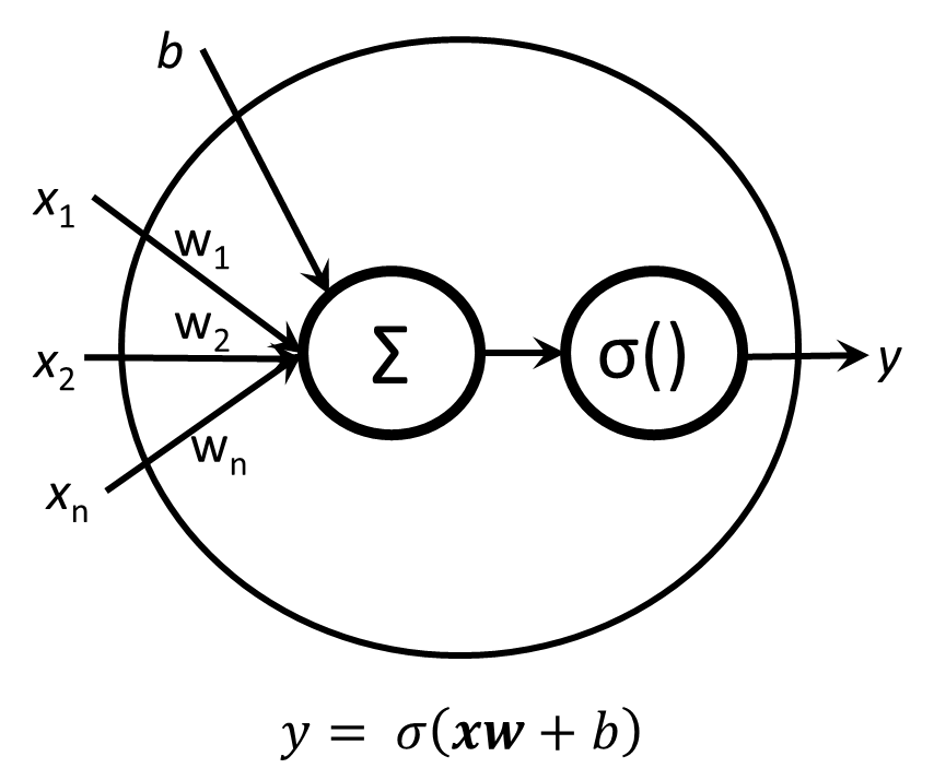
\includegraphics[width=.7\columnwidth]{images/node.png}  %assumes jpg extension
	\caption{Basic node used in most machine learning architectures }
	\label{fig:node}
\end{figure}

The basic unit of machine learning is a node as shown in  Figure \ref{fig:node}. The canonical FFNN model consists of an input layer, a hidden layer and an output layer. Each layer is constructed from interlinked nodes that generates a value (usually between -1 and 1 or 0 and 1). The individual node model is shown in Figure \ref{fig:node}. \\

The node is based on the biological neuron, where dendrites bring in sensory information in the form of bioelectric impulses until the neuron activates and sends another signal through its outputs. The machine learning node is similar to an individual neuron in that it also sums the weighted inputs of the previous layer, sometimes with a bias, and transforms the combined sum with a non-linear activation function, $\sigma$ before producing an output that becomes the input to other nodes or an output itself. The node  equation is given by

\begin{equation}
\label{eq:perceptron}
y= \sigma(wx+b)
\end{equation}
\noindent
where $w$ is an array of weights for the connections between the previous layer and the current layer, $x$ is a vector of input values from the previous layer, and $b$ is an optional bias value. Common activation functions include the sigmoid, tanh, and relu functions. A general property for activation functions is that they normalize the output and have a continuous first order derivative that can be used during the training process \citep{Goodfellow2016}. 

When many, or thousands, of nodes are used in a machine learning architecture, they become an artificial neural network (ANN). Because of the complex interconnections and nonlinear activation functions, ANNs have been successfully used to approximate complex functions and are often called 'universal approximators' \citep{Sifaoui2008, Sonoda2017}. The basic ANN is a feed-forward neural network (FFNN) as shown in Figure \ref{fig:ffnn}. It includes an input layer that takes the input data features and distributes it to hidden layers for processing. The hidden layers due the bulk of the ANN calculations because of the interconnections between nodes. Each interconnection has a weight that can be updated or turned off. An output layer converts the final calculations into a binary category or a continuous value that may require further re-mapping.

\begin{figure}[!ht]
\centering
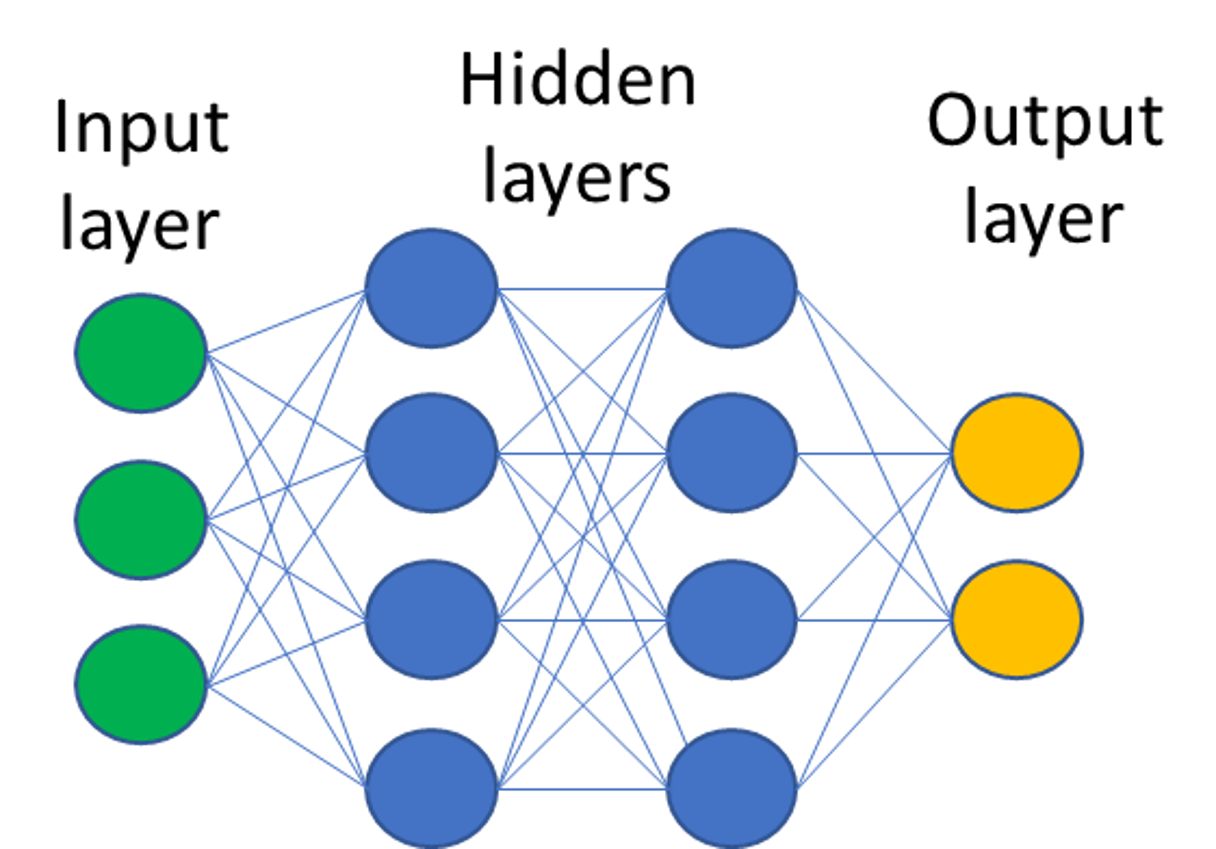
\includegraphics[width=.6\columnwidth]{images/ffnn.png}  %assumes jpg extension
\caption{Feed-forward neural network architecture}
\label{fig:ffnn}
\end{figure}
%

The benefits of using ANNs also include not requiring \textit{a priori} assumptions of the data used for training and not requiring weighting of initial inputs \citep{Gardner1998}. In practice, dimensionality reduction is often used to remove inputs to the model that are not independent and identically distributed (IID) or offer little influence to the overall training. 

Training of ANNs use gradient-based optimization to update the weights that interconnect the nodes. Through a series of back propagation, the weights are individually modified in an iterative process. The training data is then run through the network again in order to measure the error again. Each complete cycle of training is called an epoch. There is no ''one-size-fits-all'' architecture and a key challenge of using machine learning tools is selecting an appropriate architecture based on the datasets available and the desired output \citep{Wolpert1997}.

This research uses datasets generated from RANS-CFD simulations on 61 different hull designs under various conditions defined by Froude number (Fn), leeway ($\beta$), and heel angle ($\phi$) to train multi-layer neural networks in order to interpolate component forces under scenarios outside of the training set provided. 

%------------------------------------------------

\subsection{Training set: Delft Wind Assist Series}

A total set of 1,567 different RANS-CFD runs were prepared and executed over the period of 2016 and 2019 using the Numeca ISIS-CFD package. Vessel sailing performance for a range of Froude number (\Fn), leeway ($\beta$), and heel angle ($\phi$). The parameter space for hull geometry is indicated in \cref{fig:DWA} and \cref{tab:DWAsummary}.

\begin{description}[leftmargin=1cm]

\item[\TL]{Draft to lenth ratio}
\item[\Cp]{Prismatic coefficient $\frac{A_{\mathrm{Midship}}}{LBT}$}
\item[\Cm]{Midship coefficient $\frac{A_{\mathrm{Midship}}}{BT}$}
\end{description}


\begin{figure*}[!ht]
	\centering
	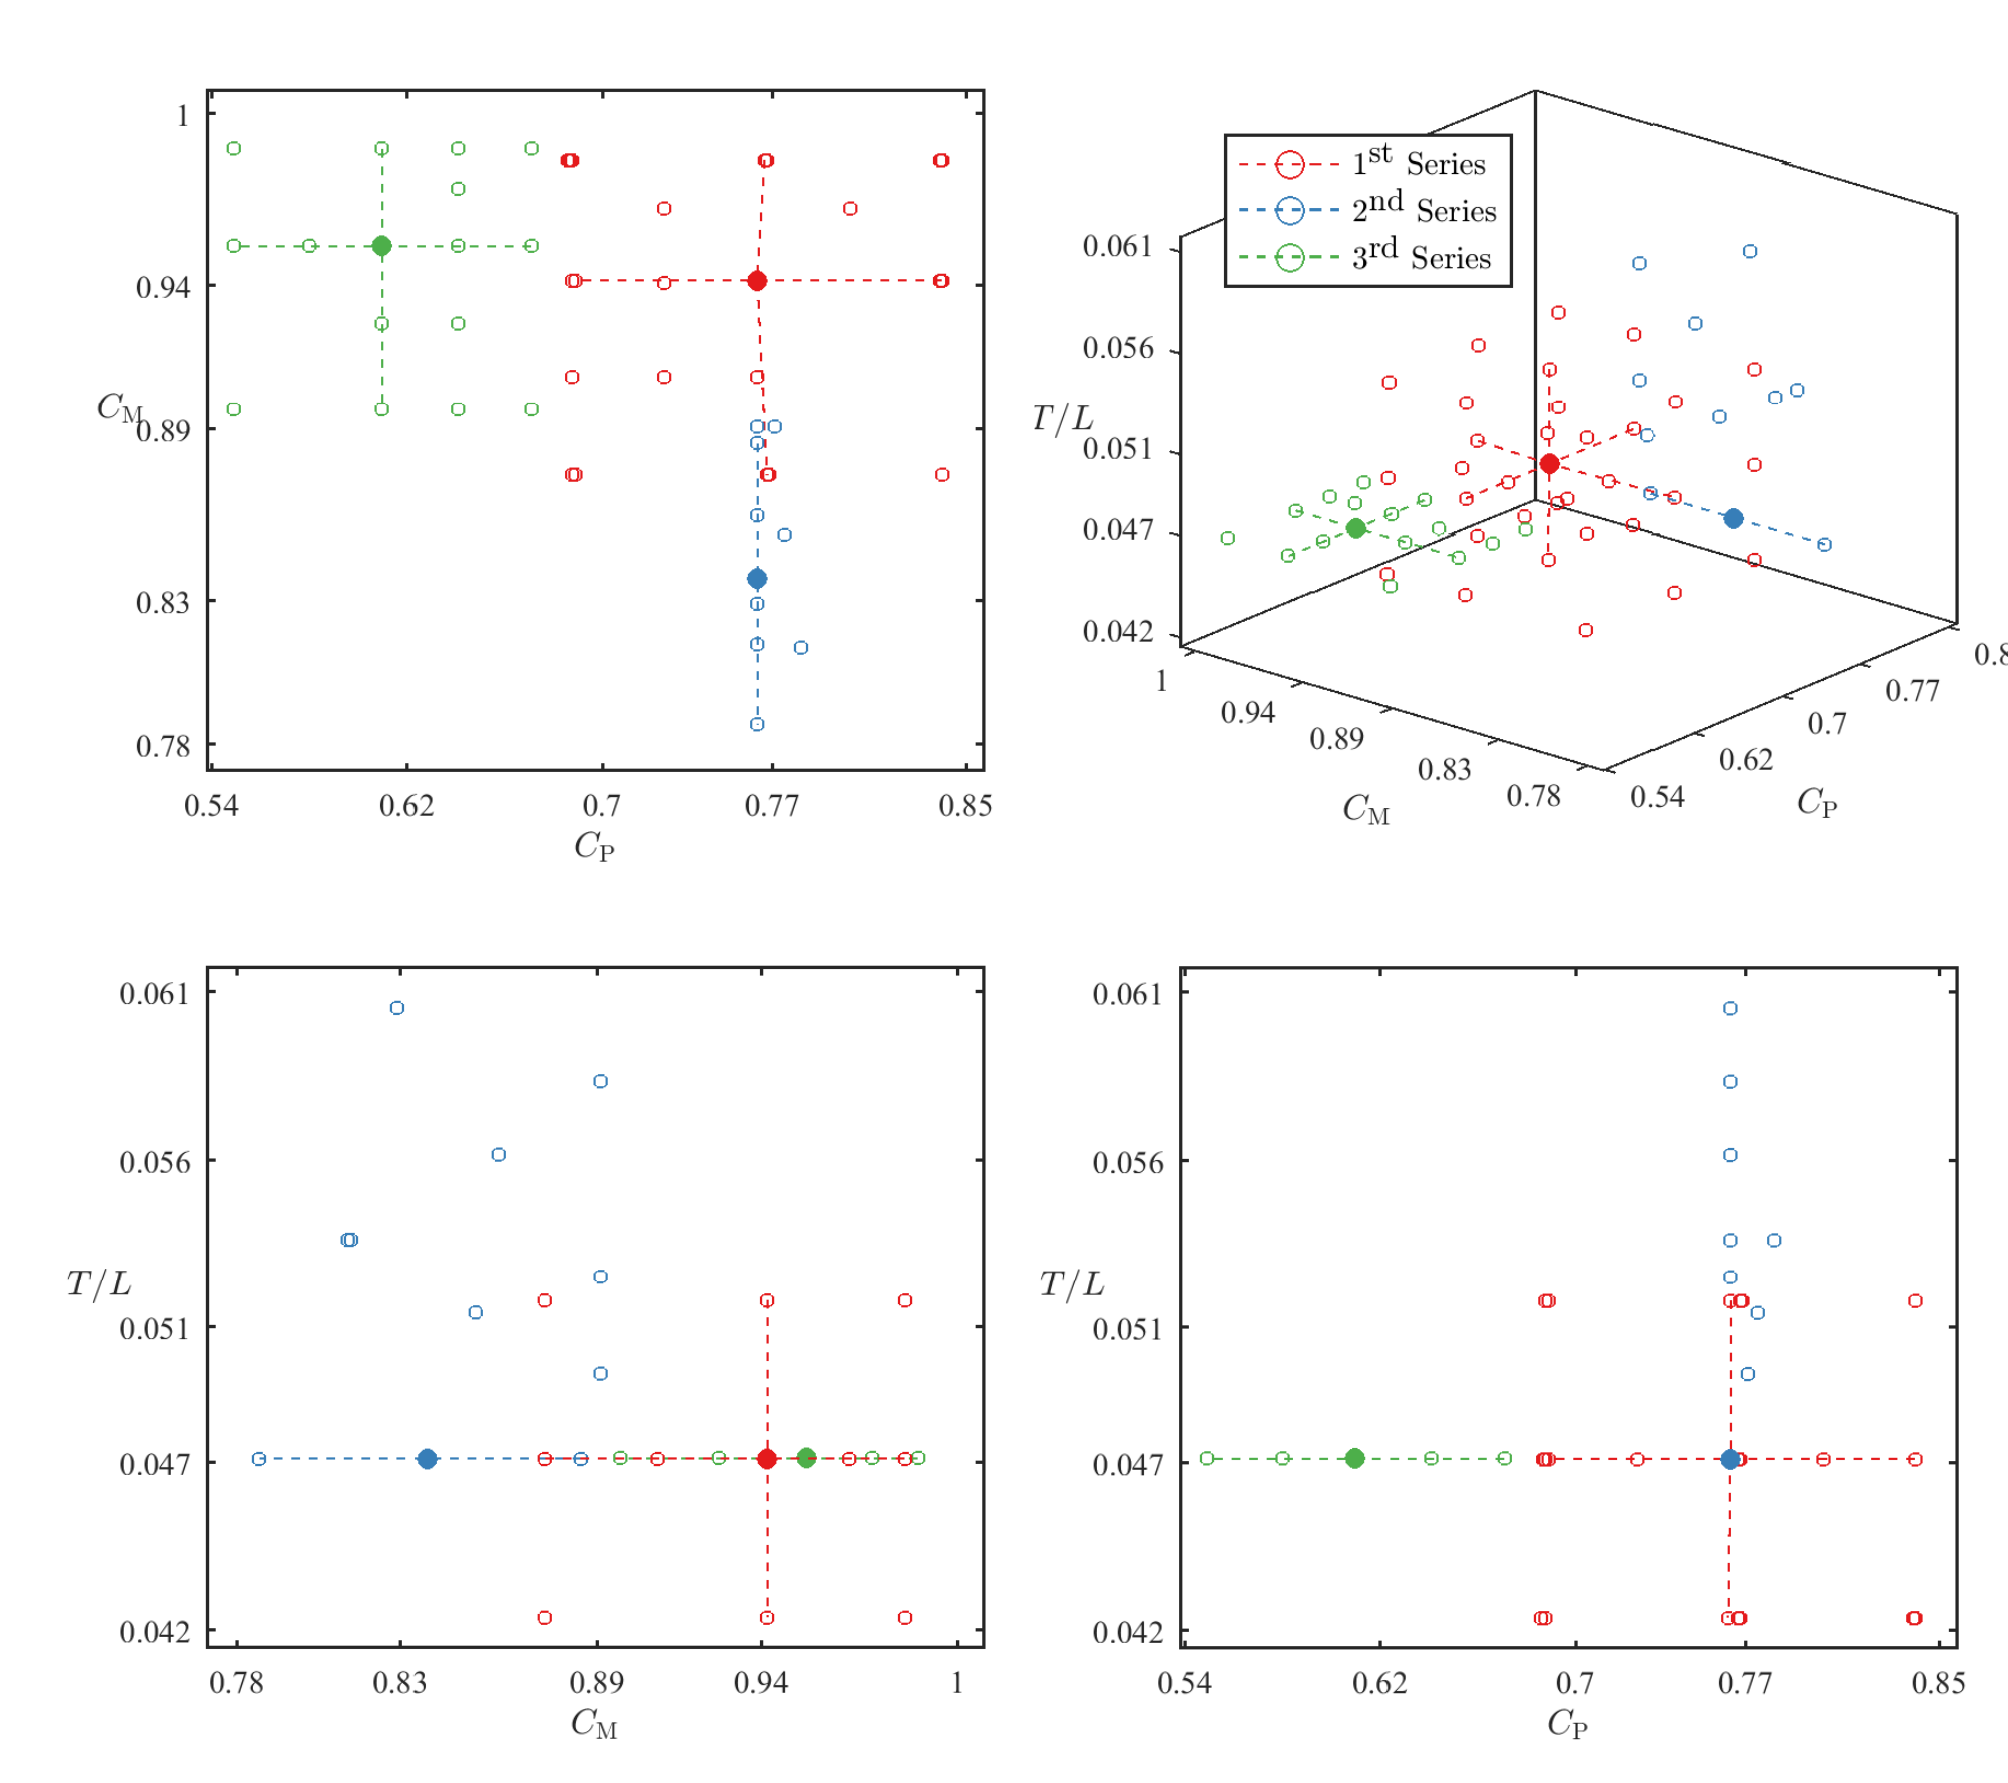
\includegraphics[width=.9\textwidth]{images/DWAseries.png}  %assumes jpg extension
	\caption{Delft wind assist series, showing main parameter variations for \TL, \Cp, and \Cm}
	\label{fig:DWA}
\end{figure*}

\begin{table}[]
	\caption{Simulation matrix for \DWA hulls}
	\label{tab:parameters}
	\begin{tabular}{@{}cc@{}}
		\toprule
		\textbf{Parameter} & \textbf{Values} \\ \midrule
		\Fn & 0.126, 0.168, 0.21 \\
		Leeway ($\beta$) & [\ang{0}-\ang{9}] \\
		Heel ($\phi$) & \ang{0}, \ang{10}, \ang{20} \\ \bottomrule
	\end{tabular}
\end{table}

The Delft Wind Assist series is a set of 60 hull forms developed by researchers at Delft University of Technology. The hull forms are  in a systematic way so that the influence of significant form coefficients for sailing behavior may be isolated and studied. The series is set up to span a design space that is presently meaningful for the application of wind-assist propulsion, summarized in \cref{tab:DWAsummary}.

The DWA is composed of three sub-series's: \\
\\ 
\leftskip = 1.5cm
\begin{tabular}[!th]{p{1.5cm}p{4cm}}
	\firstseries & Variations on the Ecoliner concept \cite{Ecoliner} \\
	\secondseries &  19\textsuperscript{th} century clipper ships \\ 
	\thirdseries & Low-\Cp \space ships (ferry, cruise, and ro-ro types) \\ 
\end{tabular}
\leftskip = 0cm

\begin{table*}[b]
	\centering
	\caption{Hydrostatics for hulls of the Delft Wind Assist Series (features of the ANN model)}
	\begin{tabular}{p{2.8cm}*{10}{S}}
		\toprule
		& {\Cb} & {\Cp} & {\Cm} & {\Cwp} & {\LB} & {\BT} & {\TL}  & {Deadrise}         \\\midrule
		\DWA ($N$=60)            &       &       &       &        &       &       &         &                    \\ \midrule
		\textit{series} $max$ & 0.827 & 0.840 & 0.988 & 0.925  & 8.44  & 3.54  & 0.061   & \ang{0}                  \\
		\textit{series} $min$ & 0.493 & 0.549 & 0.787 & 0.747  & 6.00  & 2.16  & 0.042   & \ang{0}        { \bigskip} \\
		\firstseries ($N$=33)            &       &       &       &        &       &       &         &                    \\ \midrule
		Hull 1 (Parent)                & 0.719 & 0.764 & 0.942 & 0.883  & 7.67  & 2.77  & 0.047   & \ang{0}                  \\
		\textit{series} $max$     & 0.827 & 0.840 & 0.984 & 0.925  & 8.44  & 3.42  & 0.052   & \ang{0}                  \\
		\textit{series} $min$     & 0.601 & 0.686 & 0.874 & 0.832  & 6.90  & 2.29  & 0.042   & \ang{0}        { \bigskip} \\
		\secondseries ($N$=11)            &       &       &       &        &       &       &         &                    \\ \midrule
		Hull 34 (Parent)               & 0.641 & 0.764 & 0.838 & 0.883  & 7.67  & 2.77  & 0.047   & \ang{10}                 \\
		\textit{series} $max$     & 0.687 & 0.782 & 0.891 & 0.890  & 7.67  & 2.77  & 0.061   & \ang{14}                 \\
		\textit{series} $min$     & 0.602 & 0.764 & 0.787 & 0.874  & 7.67  & 2.16  & 0.047   & \ang{6 }       { \bigskip} \\
		\thirdseries ($N$=15)            &       &       &       &        &       &       &         &                    \\ \midrule
		Hull 45 (Parent)               & 0.582 & 0.610 & 0.954 & 0.805  & 6.00  & 3.54  & 0.047   & \ang{0 }                 \\
		\textit{series} $max$     & 0.663 & 0.671 & 0.988 & 0.841  & 6.00  & 3.54  & 0.047   & \ang{0}                  \\
		\textit{series} $min$     & 0.493 & 0.549 & 0.897 & 0.747  & 6.00  & 3.54  & 0.047   & \ang{0 }                 \\ \bottomrule
	\end{tabular}
	\label{tab:DWAsummary}
\end{table*}

A multi-layer feed-forward neural network was prepared in Python 3.7 using the Keras library. Hyper parameters of the FFNN are shown in Table \ref{tab:network_parameters}.

\begin{table}[]
\caption{Network hyperparameters used to build the feed forward neural network}
\label{tab:network_parameters}
\resizebox{\columnwidth}{!}{%
\begin{tabular}{@{}lc@{}}
\toprule
\textbf{Neural Network Parameter} & \textbf{Value} \\ \midrule
Hidden layers & 2 \\
Hidden layer nodes & 114 \\
Input and hidden layer activation function & relu \\
Output activation function & tanh \\
learning rate ($\alpha_{lr}$) & 0.002 \\
Optimizer & Nesterov Adam (Nadam) \\
Loss Function & Mean Square Error \\
Dropout & 0.01 \\
Batches & 8 \\ \bottomrule
\end{tabular}
}
\end{table}

The number of hidden nodes was 6 times the input vector size (19 input features) in order to manage the complexity of the CFD output \results. A low dropout (1\%) was used instead of 10-20\% to allow more training. Dropout is a technique that addresses overfitting, or over learning the training data, by randomly removing connections from the network forcing the training to generalize the results \cite{Srivastava2014}. By reducing the dropout rate, we allowed the network to overfit under the assumption that the input parameters correlated to linear results in the CFD model.

Input parameters were normalized by dividing each value within the parameter column with the  maximum value of the column. Heel and leeway angles were converted into cosine and sine components.  Output values were multiplied by a factor of 100 to raise the small fractional values closer to 1 and then remapped using a MinMax scaler. Sequential order was not required for training so the dataset was randomly shuffled as a whole and the split into training and testing sets. A total of 85\% of the values were used for training and validating with 15\% reserved to test the trained network. 

%------------------------------------------------

\section{Results}
The model was trained for 200 epochs in which all the training data was fed to the network in batches of 8 observations before the weights were allowed to update using the average error (loss) of the batch. Of the 85\% of the total observations used for training, 15\% was used to validate the accuracy of the model after each epoch. A summary of the data breakdown is shown in Table \ref{tab:data}.

\begin{table}[]
\centering
\caption{Breakdown of data used for network training}
\label{tab:data}
\begin{tabular}{@{}cc@{}}
\toprule
\textbf{Reserved Task} & \textbf{Observations} \\ \midrule
Training data & 1136 \\
Validation data & 201 \\
Testing data & 237 \\ \bottomrule
\end{tabular}
\end{table}

The network accuracy increased steadily over the first 20 epochs as shown in Figure \ref{fig:ffnn_training}. Both training and validation accuracies stayed constant with gradual improvement over the rest of the training cycle with losses oscillating around a central value after 100 epochs. The overall training accuracy of the network was calculated as 94.9\%.
 
\begin{figure*}[!ht]
	\centering
	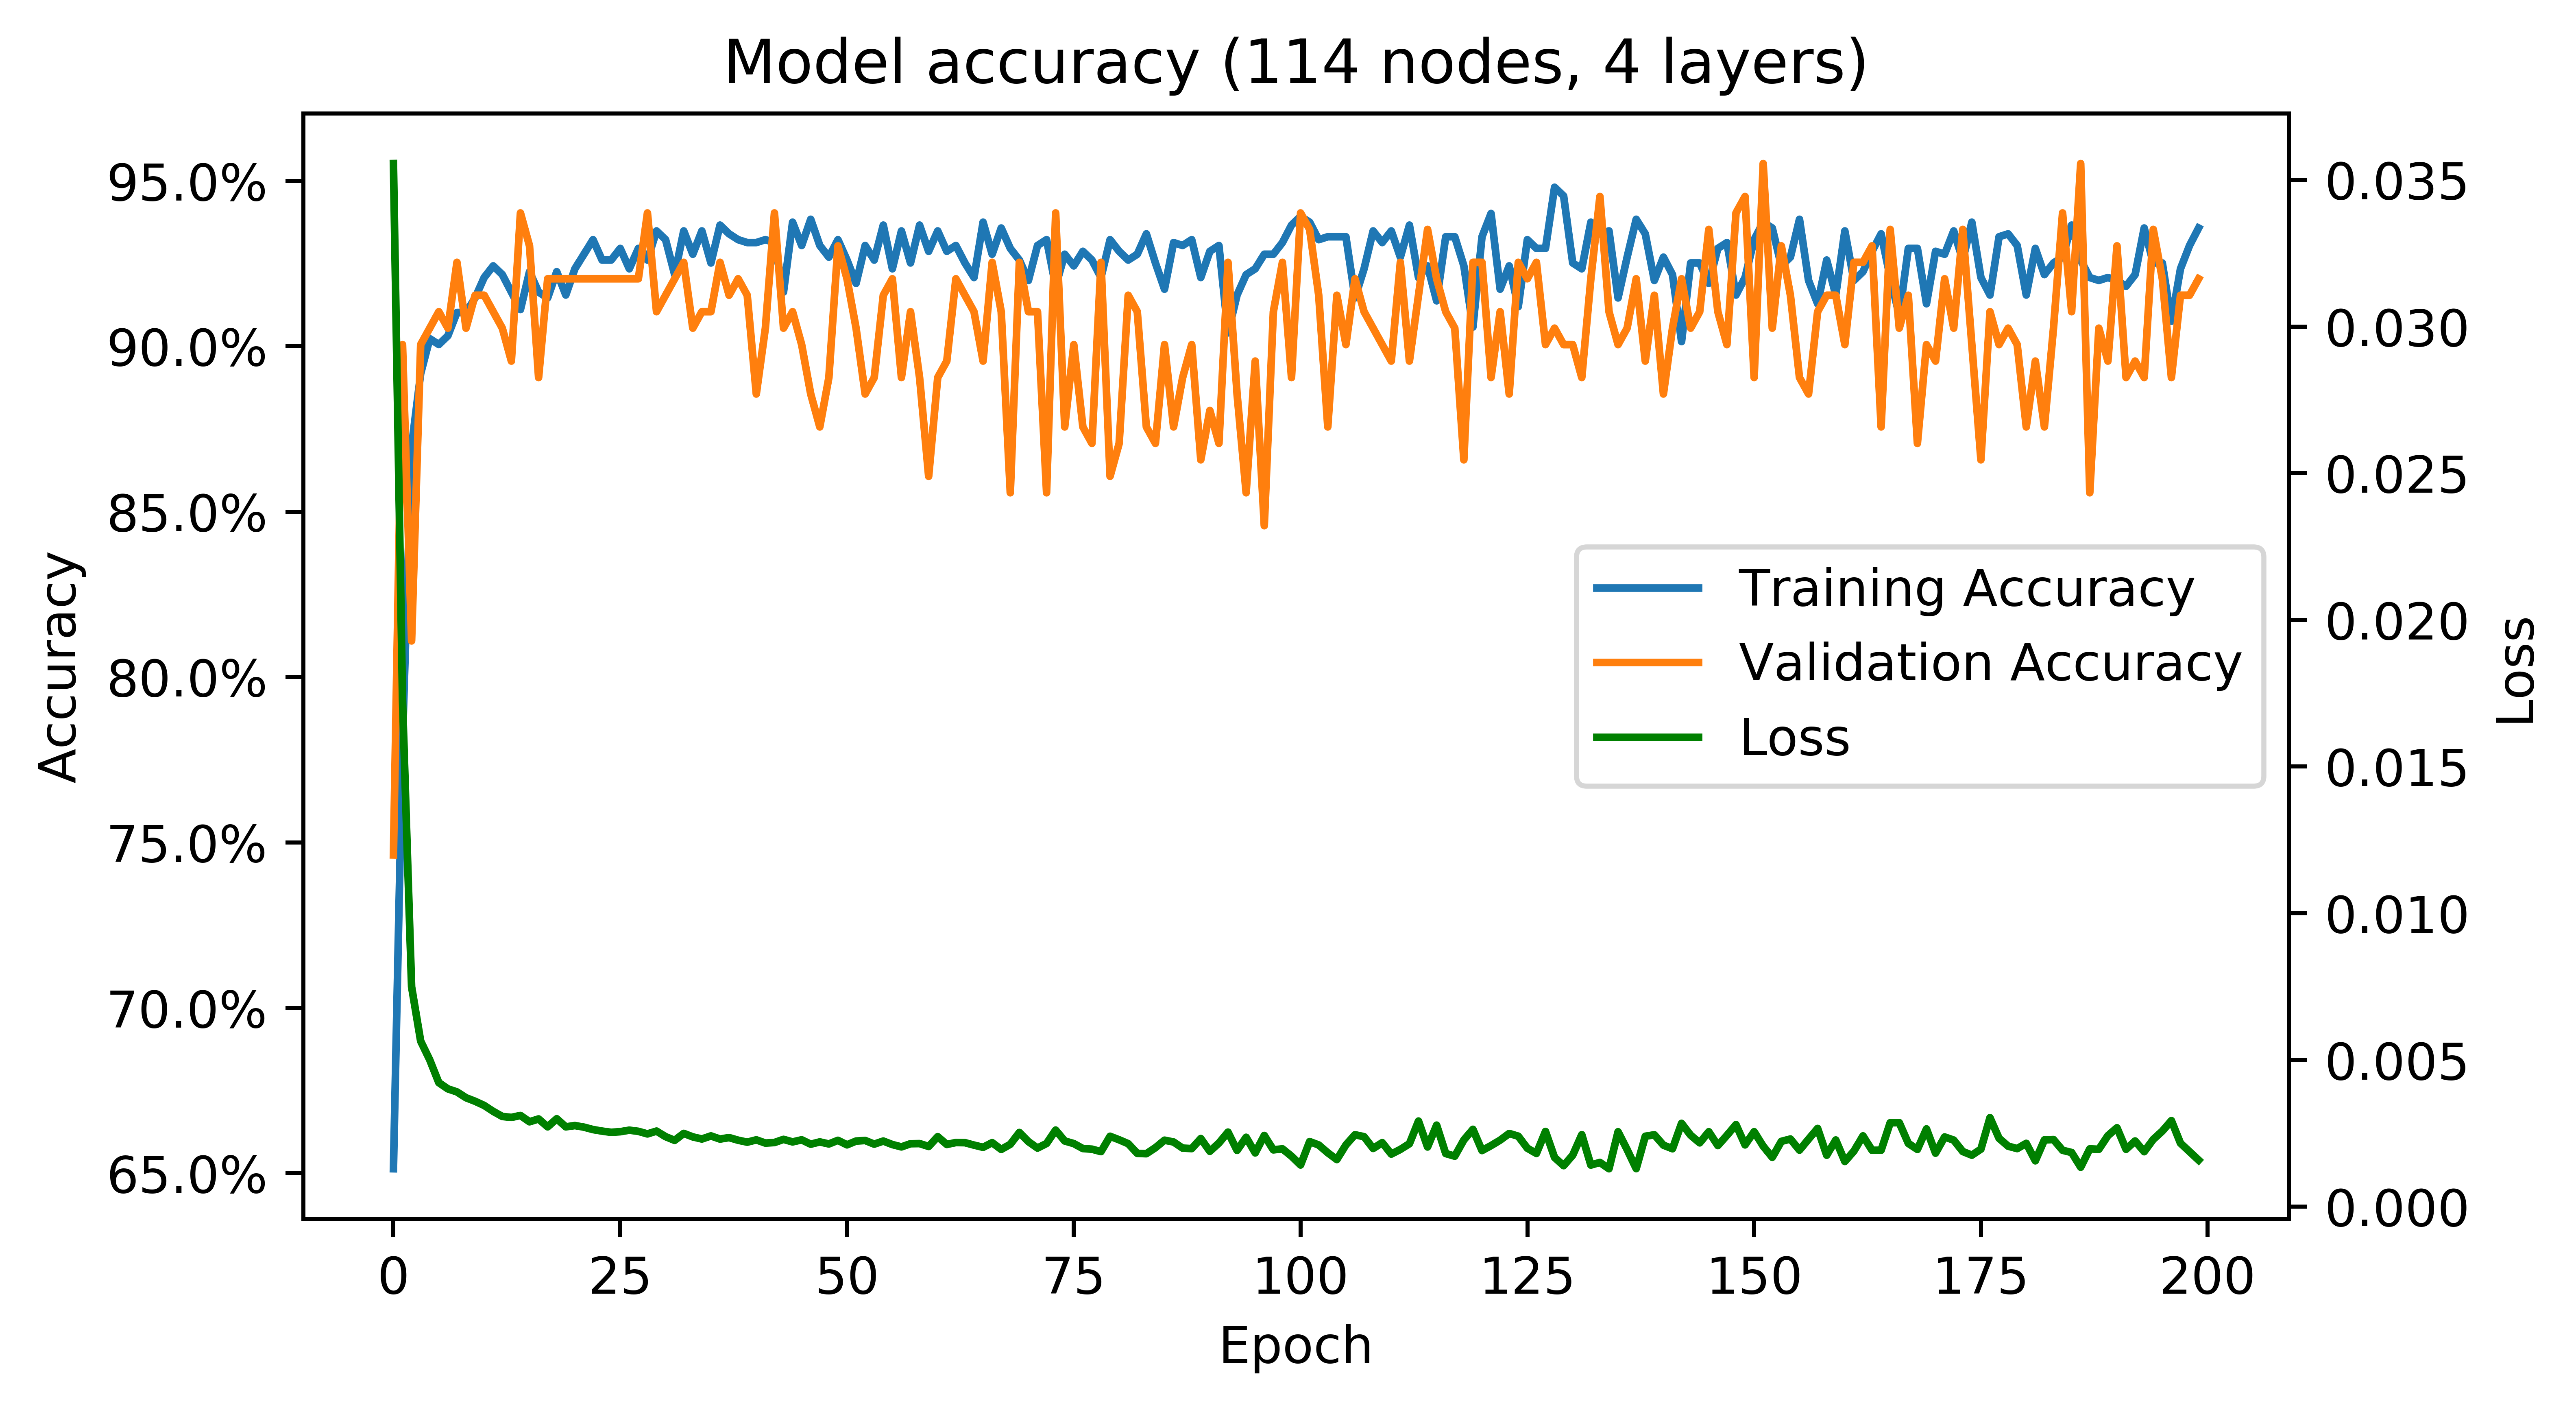
\includegraphics[width=.9\textwidth]{images/training_acc_loss.png}  
	\caption{Training accuracies of FFNN after 200 epochs showing validation accuracy and loss.}
	\label{fig:ffnn_training}
\end{figure*}

Applying the reserved test data to the trained model showed some error as measured using Mean Absolute Percent Error (MAPE) given as 

\begin{equation}
M = \frac{1}{n}\sum_{i=1}^{n}\left | \frac{A_{i}-P_{i}}{A_{i}} \right |
\end{equation}
\noident
where $A$ is the CFD modeled value and $P$ is the network predicted value. MAPE results for each force component is shown in Table \ref{tab:test_results}. The network error was considered to be within the CFD generated error.

\begin{table}[]
\centering
\caption{MAPE of the trained network using reserved test data.}
\label{tab:test_results}
\begin{tabular}{@{}ccccc@{}}
\toprule
\textbf{Component} & \textbf{Xn} & \textbf{Yn} & \textbf{Nn} & \textbf{Total} \\ \midrule
MAPE & 12.9\% & 17.2\% & 42.2\% & 24.1\% \\ \bottomrule
\end{tabular}
\end{table}

\subsection{Test Case - Hull 1}
One of the objectives of the applying a machine learning solution to CFD generated data is to provide finer resolution for operational runs in between CFD runs. Each CFD model run can be assumed to take 4-6 hrs of computational time depending on the model, complexity and processing power. As a test case, the resolution between runs used to generate the initial training set for Hull 1 was expanded. The initial scenarios of 63 cases was increased to 630 by increasing the leeway and heel angles. The hull parameters and froud numbers were left unchanged. 

The input observations were generated and processed using the same maximum column values used for the original training data and applied to the pre-trained network. The results were generated almost instantly as compared to waiting 105 days to run the 630 models individually. The average error for the different runs was 13.2\% with the individual components shown in Table \ref{tab:hull1_results}.

\begin{table}[]
\centering
\caption{MAPE results applying Hull 1 parameters to the trained network}
\label{tab:hull1_results}
\begin{tabular}{@{}ccccc@{}}
\toprule
\textbf{Component} & \textbf{Xn} & \textbf{Yn} & \textbf{Nn} & \textbf{Total} \\ \midrule
MAPE & 17.5\% & 15.5\% & 6.7\% & 13.2\% \\ \bottomrule
\end{tabular}
\end{table}

The differing errors of the individual hull compared to the average error for all 60 different hulls in Table \ref{tab:test_results} suggests that different hulls have higher error rates than other. This must be investigated in order to identify how the network accommodates variation within hull design


%------------------------------------------------

\section{Discussion}

A feed forward neural network was 


%----------------------------------------------------------------------------------------
%	REFERENCE LIST
%----------------------------------------------------------------------------------------

\bibliography{dwas-bib}{}
\bibliographystyle{plain}

%----------------------------------------------------------------------------------------
\section{AUTHORS BIOGRAPHY}

Brief biographies are required for all authors e.g.:

\textbf{B. Freeman}is a Senior Project Manager at Lakes Software.  He is responsible for researching new machine learning applications and conducting complex air dispersion modeling using CFD methods.  He holds a Ph.D. in Environmental Engineering from the University of Guelph, Canada. His current interests includes deep learning analysis of spatio-temporal events and multi-sensor integration.

\textbf{N. van der Kolk} holds the current position of [job title] at [name of organisation].  He is responsible for [brief job description].  His previous experience includes [previous experience relevant to the paper], etc.

% That's all folks!


\end{document}
